\chapter{Sorting}
In this chapter, we present various algorithms for solving the \blue{sorting problem}.
After a precise definition of the sorting problem, we start with a simple algorithm
that is very easy to implement: \blue{insertion sort}.  However, the
efficiency of this algorithms is far from optimal.  Next, we present \blue{quick sort} and 
\blue{merge sort}.  Both of these algorithms are very efficient when implemented carefully.
However, the implementation of these algorithms is considerably more involved.
After that we show that any sorting algorithm that needs to compare the elements in order to sort them will
perform $\Omega\bigl(n \cdot \log_2(n)\bigr)$ comparisons.  The last algorithm presented is \blue{radix sort}, which is an
algorithm of linear complexity for sorting numbers of a fixed size.
Finally, we show how sorting is used in the \blue{$k$-nearest-neighbour-algorithm}.
This algorithm is then used for the recognition of hand written digits.

\section{The Sorting Problem}
In this chapter, we assume that we have been given a list $L$.  The elements of $L$ are members of
some set $S$.  If we want to \blue{sort} the list $L$ we have to be able to compare these elements
to each other.   Therefore, we assume that $S$ is equipped with a binary relation $\leq$ which is
\blue{reflexive}\index{reflexive}, \blue{anti-symmetric}\index{anti-symmetric}, and
\blue{transitive}\index{transitive}, i.~e.~we have   
\begin{enumerate}
\item $\forall x \el S \colon x \leq x$,                      \hspace*{\fill} ($\leq$ is reflexive)
\item $\forall x, y \el S \colon \bigl(x \leq y \wedge y \leq x
  \rightarrow x = y\bigr)$,   \hspace*{\fill} ($\leq$ is anti-symmetric)
\item $\forall x, y, z \el S \colon \bigl(x \leq y \wedge y \leq z \rightarrow x \leq z\bigr)$.  \hspace*{\fill} ($\leq$ is transitive)
\end{enumerate}
\begin{Definition}[Linear Order\label{def:linear_order}] \index{linear order}
  A pair $\langle S, \leq \rangle$ where $S$ is a set and $\leq \;\subseteq S \times S$ is a relation
  on $S$ that is \blue{reflexive}, \blue{anti-symmetric} and \blue{transitive} is called a
  \href{http://en.wikipedia.org/wiki/Partially_ordered_set}{partially ordered set}\index{partially ordered set}.  
  If, furthermore
  \\[0.2cm]
  \hspace*{1.3cm}
  $\forall x, y \el S \colon\bigl( x \leq y \vee y \leq x\bigr)$
  \\[0.2cm]
  holds, then the pair $\langle S, \leq \rangle$ is called a 
  \href{http://en.wikipedia.org/wiki/Totally_ordered_set}{totally ordered set} and
  the relation $\leq$ is called a \blue{total order} or a \blue{linear order}\index{linear order}. \eox
\end{Definition}

\examples
\begin{enumerate}
\item $\langle\mathbb{N}, \leq \rangle$ is a totally ordered set.
\item $\langle 2^{\mathbb{N}}, \subseteq \rangle$ is a partially ordered set, but it is not a totally
      ordered set.  For example, the sets $\{1\}$ and $\{2\}$ are not comparable since we have
      \\[0.2cm]
      \hspace*{1.3cm}
      $\{1\} \not\subseteq \{2\}$ \quad and \quad  $\{2\} \not\subseteq \{1\}$.
\item If $P$ is the set of employees of some company and if we define for two given employees
      $a,b \el P$
      \\[0.2cm]
      \hspace*{1.3cm}
      $a \preceq b$ \quad iff \quad  $a$ does not earn more money than $b$, 
      \\[0.2cm]
      then the pair $\langle P, \leq \rangle$ is not a partially ordered set.  The reason is that
      the relation $\preceq$ is not anti-symmetric:  If Mr.~Smith earns as much as
      Mrs.~Robinson, then we have both
      \\[0.2cm]
      \hspace*{1.3cm}
      $\mathrm{Smith} \preceq \mathrm{Robinson}$ \quad and \quad $\mathrm{Robinson} \preceq \mathrm{Smith}$
      \\[0.2cm]
      but obviously $\mathrm{Smith} \not= \mathrm{Robinson}$.
\end{enumerate}
In the example given above we see that it does not make much sense to sort subsets of $\mathbb{N}$.
However, we can sort natural numbers with respect to their size and we can also sort employees with
respect to their income.  This shows that, in order to sort,  we do not necessarily need a totally
ordered set.  In order to capture the requirements that are needed to be able to sort we introduce
the notion of a \href{http://en.wikipedia.org/wiki/Preorder}{quasiorder}.

\begin{Definition}[Quasiorder]  \hspace*{\fill} \\
{\em
  A pair $\langle S, \preceq\rangle$ is a \href{https://en.wikipedia.org/wiki/Preorder}{quasiorder} \index{quasiorder}  iff $\preceq$ is a 
  binary relation on $S$ such that we have the following:
  \begin{enumerate}
  \item $\forall x \el S\colon x \preceq x$. \hspace*{\fill} (reflexivity)
  \item $\forall x, y, z \el S \colon \bigl(x \preceq y \wedge y \preceq z \rightarrow x \preceq z\bigr)$. 
         \hspace*{\fill} (transitivity)
  \end{enumerate}
  If, furthermore,
  \\[0.2cm]
  \hspace*{1.3cm}
  $\forall x, y \el S \colon \bigl(x \preceq y \vee y \preceq x\bigr)$ \hspace*{\fill} (linearity) \index{linearity}
  \\[0.2cm]
  holds, then $\langle S, \preceq \rangle$ is called a \blue{total quasiorder}.  This will be
  abbreviated as \textsc{TQO}.
}
\end{Definition}
A quasiorder $\langle S, \preceq \rangle$ does not require the relation $\preceq$ to be
anti-symmetric.  Nevertheless, the notion of a quasiorder is very closely related to the notion of a
linear order.  The reason is as follows:  If $\langle S, \preceq \rangle$ is a quasiorder, then we can define an
\href{https://en.wikipedia.org/wiki/Equivalence_relation}{equivalence relation}\index{equivalence relation}\footnote{
  A pair $\langle M, \approx \rangle$ where $M$ is a set and $\approx$ is a binary relation on $M$ called an
  \blue{equivalence relation on $M$} iff we have
  \begin{enumerate}[(a)]
  \item $\forall x \el M \colon x \approx x$,                      \hspace*{\fill} ($\approx$ is reflexive)
  \item $\forall x, y \el M \colon \bigl(x \approx y \rightarrow y \approx x\bigr)$,
        \hspace*{\fill} ($\approx$ is symmetric)
  \item $\forall x, y, z \el M \colon \bigl(x \approx y \wedge y \approx z \rightarrow x \approx z\bigr)$.
        \hspace*{\fill} ($\approx$ is transitive)
\end{enumerate}
}
$\approx$ on $S$ by setting
\\[0.2cm]
\hspace*{1.3cm}
$x \approx y \stackrel{\mbox{\scriptsize def}}{\Longleftrightarrow} x \preceq y \wedge y \preceq x$. 
\\[0.2cm]
If we extend the order $\preceq$ to the equivalence classes generated by the relation $\approx$,
then it can be shown that this extension is a linear order.
\vspace*{0.3cm}

Let us assume that $\langle M, \preceq \rangle$ is a  \textsc{TQO}.
Then the \blue{sorting problem}\index{sorting problem} is defined as follows:
\begin{enumerate}
\item A list $L$ of elements of $M$ is given.
\item We want to compute a list $S$ such that we have the following: 
  \begin{enumerate}
  \item $S$ is sorted \blue{ascendingly}\index{sorted ascendingly}, i.e.~we have: \\[0.2cm]
        \hspace*{1.3cm} 
        $\forall i \el \{ 0, \cdots, \mytt{len}(S)-2 \} \colon S[i] \preceq S[i+1]$ 
        \\[0.2cm]
        Here, the length of the list $S$ is denoted as $\mytt{len}(S)$ and $S[i]$ is the element at position
        $i$ in $S$.  We assume here that the first position is indexed with index $0$.
  \item The elements of $M$ occur in $L$ and $S$ with the same frequency: \\[0.2cm]
        \hspace*{1.3cm} 
        $\forall x\el M \colon \textsl{count}(x,L) = \textsl{count}(x,S)$.
        \\[0.2cm]
        Here, the function $\textsl{count}(x,L)$ returns the number of occurrences of $x$ in $L$.
        Therefore,  \\[0.2cm]
        \hspace*{1.3cm}
        $\textsl{count}(x,L) := \mytt{card}\bigl(\bigl\{ i \el \{0,\cdots,\mytt{len}(L)-1\} \mid L[i] = x \bigr\}\bigr)$.
        \\[0.2cm]
        Sometimes, this second requirement is changed as follows:
        \\[0.2cm]
        \hspace*{1.3cm}
        $\forall x \in S: \textsl{count}(x,S) \leq 1 \wedge \forall x\el M \colon \bigl(\textsl{count}(x,L) > 0 \leftrightarrow \textsl{count}(x,S) = 1\bigr)$.
        \\[0.2cm]
        Hence, in this case we require that the sorted list $s$ does not contain
        \blue{duplicate elements}\index{duplicate elements}.
        Of course, an object $x$ should only occur in $S$ if it also occurs in $L$.  If we change
        the second requirement in this way, then the main purpose of sorting is to remove \blue{duplicate}
        elements from a list.  This is actually a common application of sorting in practice.  The
        reason this application is so common is that a list that contains every element at
        most once can be regarded as a set.
  \end{enumerate}
\end{enumerate}

\exercise
Assume a list $S$ is sorted and contains every object at most once.  Develop an efficient
algorithm for testing whether a given object $x$ is a member of the list $S$.

\hint Try to develop an algorithm that follows the \blue{divide-and-conquer}
paradigm. 
\eoxs

\section{Insertion Sort \label{sec:insertionSort}}
Let us start our investigation of sorting algorithms with the algorithm
\href{http://en.wikipedia.org/wiki/Insertion_sort}{insertion sort}\index{insertion sort}.
We will describe this algorithm via a set of equations.
\begin{enumerate}
\item If the list $L$ that has to be sorted is empty, then the result is the empty list: 
      \\[0.2cm]
      \hspace*{1.3cm}
      $\mytt{sort}([]) = []$.
\item Otherwise, the list $L$ must have the form $[x] + R$. Here, $x$ is the first element of $L$
      and $R$ is the rest of $L$, i.e.~everything of $L$ but the first element.  In order to sort
      $L$ we first sort the rest $R$ and then we \blue{insert} the element $x$ into the resulting list in a
      way that the resulting list remains sorted:
      \\[0.2cm]
      \hspace*{1.3cm} $\mytt{sort}\bigl([x] + R\bigr) = \mytt{insert}\bigl(x, \mytt{sort}(R)\bigr)$.
\end{enumerate}
Inserting $x$ into an already sorted list $S$ is done according to the following specification:
\begin{enumerate}
\item If $S$ is empty, the result is the list $[x]$: \\[0.2cm]
      \hspace*{1.3cm}
      $\mytt{insert}(x,[]) = [x]$.
\item Otherwise, $S$ must have the form $[y] + R$.  In order to know where to insert $x$ we have to
      compare $x$ and $y$.
      \begin{enumerate}
      \item If $x \preceq y$, then we can insert $x$ at the front of the list $S$: \\[0.2cm]
            \hspace*{1.3cm}
            $x \preceq y \rightarrow \mytt{insert}\bigl(x, [y] + R\bigr) = [x,y] + R$. 
      \item Otherwise, $x$ has to be inserted recursively into the list $R$: \\[0.2cm]
            \hspace*{1.3cm}
            $\neg x \preceq y \rightarrow \mytt{insert}\bigl(x, [y] + R\bigr) = [y] + \mytt{insert}(x,R)$. 
      \end{enumerate}
\end{enumerate}

\begin{figure}[!ht]
  \centering
\begin{minted}[ frame         = lines, 
                framesep      = 0.3cm,
                bgcolor       = sepia,
                numbers       = left,
                numbersep     = -0.2cm,
                xleftmargin   = 0.3cm,
                xrightmargin  = 0.3cm
              ]{python3}
    def sort(L):
        if L == []:
            return []
        x, *R = L
        return insert(x, sort(R))
        
    def insert(x, L):
        if L == []:
            return [x]
        y, *R = L
        if x <= y:
            return [x] + L
        else:
            return [y] + insert(x, R)
\end{minted}
\vspace*{-0.3cm}
  \caption{Implementing \blue{insertion sort} in \textsl{Python}.}
  \label{fig:Insertion-Sort.ipynb}
\end{figure} 

\noindent
Figure \ref{fig:Insertion-Sort.ipynb} shows how the \blue{insertion-sort} algorithm can be implemented 
in \textsl{Python}.
\begin{enumerate}
\item If $\mytt{L}$ is empty, we return the empty list.
\item Otherwise, the assignment
      \\[0.2cm]
      \hspace*{1.3cm}
      \mytt{x, *R = L}
      \\[0.2cm]
      splits $\mytt{L}$ into two parts: $\mytt{x}$ is the first element of $\mytt{L}$ and $\mytt{R}$ is the rest of $\mytt{L}$,
      i.e.~all elements of $\mytt{L}$ with the exception of the first element.  Next, the rest $\mytt{R}$
      is sorted and $\mytt{x}$ is inserted into $\mytt{R}$.
\item In order to insert $\mytt{x}$ into a list $\mytt{L}$ that is already sorted, we first check whether
      $\mytt{L}$ is the empty list.  Inserting $\mytt{x}$ into the empty list yields the list $[\mytt{x}]$.
\item Otherwise, $\mytt{L}$ is split into two parts: $\mytt{y}$ is the first element of $\mytt{L}$ and
      $\mytt{R}$ is the rest of $\mytt{L}$. 
      Then, there are two cases:
      \begin{enumerate}[(a)]
      \item If $\mytt{x}$ is less or equal than $\mytt{y}$, then, as $\mytt{L}$ is sorted,  $\mytt{x}$
            is less or equal than all elements of $\mytt{L}$ and therefore $\mytt{x}$ is prepended in front
            of $\mytt{L}$. 
      \item Otherwise, we recursively insert $\mytt{x}$ into the rest $\mytt{R}$ and prepend $\mytt{y}$
            to the resulting list.     
      \end{enumerate}
\end{enumerate}

\subsection{Complexity of Insertion Sort}
We will compute the number of comparisons that are done in the implementation of \mytt{insert}
in line 7 of Figure \ref{fig:Insertion-Sort.ipynb} in the worst case if we call $\mytt{sort}(\mytt{L})$ with a list
$\mytt{L}$ of length $n$. In order to do that, 
we have to compute the number of evaluations of the operator ``\mytt{<=}'' when 
 $\mytt{insert}(\mytt{x},\mytt{L})$ is evaluated for a list $\mytt{L}$ of length $n$.  Let us denote this number as 
$a_n$.  The worst case happens if $\mytt{x}$ is bigger than every element of $\mytt{L}$ because in that case the
test ``\mytt{x <= y}'' in line 11 of Figure \ref{fig:Insertion-Sort.ipynb} will always evaluate to
\mytt{False} and therefore \mytt{insert} will keep calling itself recursively.
Then we have
\\[0.2cm]
\hspace*{1.3cm}
$a_0 = 0$ \quad and \quad $a_{n+1} = a_n + 1$. 
\\[0.2cm]
A trivial induction shows that this recurrence relation has the solution
\\[0.2cm]
\hspace*{1.3cm} 
$a_n = n$.
\\[0.2cm]
Hence, in the worst case the evaluation of $\mytt{insert}(\mytt{x},\mytt{L})$ will lead to $n$ comparisons for a list
$\mytt{L}$ of length $n$.  The reason is simple:  If $\mytt{x}$ is bigger than any element of $L$, then we have to
compare $\mytt{x}$ with every element of $\mytt{R}$ in order to insert $\mytt{x}$ into $\mytt{R}$.

Next, let us compute the number of comparisons that have to be done when calling
$\mytt{sort}(\mytt{L})$ in the worst case for a list  $\mytt{L}$ of length $n$.  Let us denote this number as
$b_n$. The worst case happens if $\mytt{L}$ is already sorted in reverse order, i.e.~if $\mytt{L}$ is
\blue{sorted descendingly}\index{sorted descendingly}, because then the element $\mytt{x}$ that is inserted in
$\mytt{sort}(\mytt{R})$ is bigger than all elements 
of $\mytt{R}$ and therefore also bigger than all elements of $\mytt{sort}(\mytt{R})$.  Then we have \\[0.2cm]
\hspace*{1.3cm}
 $b_0 = 0$ \quad and \quad $b_{n+1} = b_n + n$, \hspace*{\fill} (1)
\\[0.2cm]
because for a list of the form $\mytt{L} = [x] + \mytt{R}$ of length $n+1$ we first have to sort the list $\mytt{R}$
recursively.  As $\mytt{R}$ has length $n$ this takes $b_n$ comparisons.  After that, the call
$\mytt{insert}(\mytt{x}, \mytt{sort(\mytt{R})})$ 
inserts the element $\mytt{x}$ into $\mytt{sort}(\mytt{R})$.  We have previously seen that this takes $n$
comparisons if $\mytt{x}$ is bigger than all elements of $\mytt{sort}(\mytt{R})$ and if the list $\mytt{L}$ is sorted
descendingly this will indeed be the case.

If we substitute $n$ by $n-1$ in equation $(1)$ we find
\\[0.2cm]
\hspace*{1.3cm}
$b_n = b_{n-1} + (n - 1)$.
\\[0.2cm]
This recurrence equation is solved by expanding the right hand side successively as follows:
\\[0.2cm]
\hspace*{1.3cm}
$
\begin{array}[t]{lcl}
  b_{n} & = & b_{n-1} + (n - 1)                     \\ 
        & = & b_{n-2} + (n - 2) + (n - 1)           \\ 
        & \vdots &                                  \\
        & = & b_{n-k} + (n - k) + \cdots + (n - 1)  \\ 
        & \vdots &                                  \\
        & = & b_{0} + 0 + \cdots + (n - 1)      \\[0.2cm] 
        & = & \ds b_{0} + \sum\limits_{i = 0}^{n - 1} i \\[0.4cm]
        & = & \frac{1}{2} \cdot n \cdot (n - 1),
\end{array}
$
\\[0.2cm]
because the sum of all natural numbers from 0 up to  $n - 1$ is given as
\\[0.2cm]
\hspace*{1.3cm}
$\ds\sum\limits_{i = 0}^{n - 1} i  = \frac{1}{2} \cdot n \cdot (n - 1)$.
\\[0.2cm]
This last formula can be shown by a straightforward induction.  Therefore, in the worst case the number $b_n$ of
comparisons needed for sorting a list of length $n$  satisfies 
\\[0.2cm]
\hspace*{1.3cm}
$\ds b_n = \frac{1}{2} \cdot n^2 - \frac{1}{2} \cdot n = \frac{1}{2} \cdot n^2 + \Oh(n)$.
\\[0.2cm]
Therefore, in the worst case the number of comparisons is given as $\Oh(n^2)$ and hence
\blue{insertion sort} has a \blue{quadratic} complexity.


Next, let us consider the best case.  The best case happens if the list $L$ is already sorted
ascendingly.  Then, the call of 
$\mytt{insert}(\mytt{x},\mytt{sort}(\mytt{R}))$ needs a single comparison provided $\mytt{R}$ is non-empty.  This time, the recurrence
equation for the number $b_l$ of comparisons when sorting $\mytt{L}$ satisfies
 \\[0.2cm]
\hspace*{1.3cm}
$b_1 = 0$ \quad and \quad $b_{n+1} = b_n + 1$. 
\\[0.2cm]
Obviously, the solution of this recurrence equation is $b_n = n-1$.  Therefore, in the best case
\blue{insertion sort} has a \blue{linear} complexity.  This is as good as it can possibly get because when
sorting a list $\mytt{L}$ we must at least inspect all of the elements of $\mytt{L}$ and therefore we will
always have at least a linear amount of work to do.


% \section{Selection Sort$^*$}
% Next, we discuss 
% \href{http://en.wikipedia.org/wiki/Selection_sort}{selection sort}\index{selection sort}.  In order to sort a
% given list $\mytt{L}$ this algorithm works as
% follows:
% \begin{enumerate}
% \item If $\mytt{L}$ is empty, the result is the empty list: \\[0.2cm]
%       \hspace*{1.3cm} $\mytt{sort}\bigl([]\bigr) = []$.
% \item Otherwise, we compute the smallest element of the list $\mytt{L}$ and we remove this element from
%       $\mytt{L}$.  Next, the remaining list is sorted recursively.  Finally, the smallest element is added
%       to the front of the sorted list:
%       \\[0.2cm]
%       \hspace*{1.3cm} 
%       $\mytt{L} \not= [] \wedge \mytt{x} := \min(\mytt{L}) \rightarrow \mytt{sort}\bigl(\mytt{L}\bigr) = [\mytt{x}] + \mytt{sort}\bigl(\mytt{delete}(\mytt{x}, \mytt{L})\bigr)$.
% \end{enumerate}
% The algorithm to delete an element $\mytt{x}$ from a list $\mytt{L}$ is also formulated recursively.  There are three cases:
% \begin{enumerate}
% \item If $\mytt{L}$ is empty, we have \\[0.2cm]
%       \hspace*{1.3cm} $\mytt{delete}\bigl(\mytt{x}, []\bigr) = []$.
% \item If $\mytt{x}$ is equal to the first element of $\mytt{L}$, then the function \mytt{delete} returns the
%       rest of $\mytt{L}$: \\[0.2cm]
%       \hspace*{1.3cm} 
%       $\mytt{delete}\bigl(\mytt{x}, [\mytt{x}] + \mytt{R}\bigr) = \mytt{R}$.
% \item Otherwise, the element $\mytt{x}$ is removed recursively from the rest of the list: \\[0.2cm]
%       \hspace*{1.3cm}   
%       $\mytt{x} \not = \mytt{y} \rightarrow \mytt{delete}\bigl(\mytt{x}, [\mytt{y}] + \mytt{R}\bigr) = [\mytt{y}] + \mytt{delete}(\mytt{x},\mytt{R})$.
% \end{enumerate}
% Finally, we have to specify the computation of the minimum of a list $\mytt{L}$:
% \begin{enumerate}
% \item The minimum of the empty list is bigger than any element.  Therefore we have 
%       \\[0.2cm]
%       \hspace*{1.3cm} $\mytt{min}\bigl([]\bigr) = \infty$.
% \item In order to compute the minimum of the list $[\mytt{x}] + \mytt{R}$ we compute the minimum of $\mytt{R}$ and
%       then use the binary function $\mytt{min}$: \\[0.2cm]
%       \hspace*{1.3cm} 
%       $\mytt{min}\bigl([\mytt{x}] + \mytt{R}\bigr) = \mytt{min}\bigl(\mytt{x}, \mytt{min}(\mytt{R}) \bigr)$. 

%       Here, the binary function $\mytt{min}$ is defined as follows: \\[0.2cm]
%       \hspace*{1.3cm} 
%       $\mytt{min}(\mytt{x},\mytt{y}) = \left\{
%       \begin{array}{ll}
%         \mytt{x}  & \mbox{if $\mytt{x} \preceq \mytt{y}$;} \\
%         \mytt{y}  & \mbox{otherwise.} \\
%       \end{array}\right.
%       $
% \end{enumerate}
% Figure \ref{fig:selection-sort.setlx} on page \pageref{fig:selection-sort.setlx} shows an
% implementation of selection sort in \textsl{Python}.  There is no need to implement the function
% $\mytt{min}$ as this function is already predefined in \textsl{Python}. 
% The implementation of $\mytt{delete}(x,L)$ is \blue{defensive}:  Normally, $\mytt{delete}(x, L)$
% should only be called if $x$ is indeed an element of the list $L$.   Therefore, if the algorithm tries 
% to delete an element from the empty list, something must have gone wrong.  The \mytt{assert}
% statement will provide us with an error message in this case.  This error message is printed if $L$ is empty.

% If $L$ is not empty we check whether $x$ is the first element of $L$.  If it is, the rest of $L$ is
% returned.  Otherwise, $x$ is deleted recursively from the rest of $L$.



% \begin{figure}[!ht]
%   \centering
% \begin{minted}[ frame         = lines, 
%                 framesep      = 0.3cm, 
%                 bgcolor = sepia,
%                 numbers       = left,
%                 numbersep     = -0.2cm,
%                 xleftmargin   = 0.3cm,
%                 xrightmargin  = 0.3cm
%               ]{python3}
%     def sort(L):
%         if L == []:
%             return []
%         x = min(L)
%         return [x] + sort(delete(x, L))
    
%     def delete(x, L):
%         if L == []:
%             assert L != [], f'delete({x}, [])'
%         y, *R = L
%         if y == x:
%             return R
%         return [y] + delete(x, R)    
% \end{minted}
% \vspace*{-0.3cm}
%   \caption{Implementing \blue{selection sort} in \textsl{Python}.}
%   \label{fig:selection-sort.setlx}
% \end{figure}


% \subsection{Complexity of Selection Sort}
% In order to be able to analyse the complexity of \blue{selection sort} we have to count the number
% of comparisons that are performed when $\mytt{min}(\mytt{L})$ is computed.  We have 
% \\[0.2cm]
% \hspace*{1.3cm} 
% $\mytt{min}([x_1,x_2,x_3,\cdots,x_n]) = \mytt{min}(x_1, \mytt{min}(x_2, \mytt{min}(x_3, \cdots \mytt{min}(x_{n-1},x_n) \cdots )))$. 
% \\[0.2cm]
% Therefore, in order to compute $\mytt{min}(\mytt{L})$ for a list $\mytt{L}$ of length $n$ the binary function $\mytt{min}$
% is called $(n-1)$ times.  Each of these calls of $\mytt{min}$ causes an evaluation of the comparison
% operator ``$\preceq$''.  If the number of evaluations of the comparison operator used to sort a list
% $\mytt{L}$ of length $n$ is written as $b_n$, we have \\[0.2cm]
% \hspace*{1.3cm}
% $b_0 = 0$ \quad und \quad $b_{n+1} = b_n + n$. 
% \\[0.2cm]
% The reasoning is as follows: In order to sort a list of $n+1$ elements using selection sort we first
% have to compute the minimum of this list.  We need $n$ comparisons for this.  Next, the minimum is
% removed from the list and the remaining list, which now contains only $n$ elements, is sorted
% recursively.  We need $b_n$ evaluations of the comparison operator for this recursive invocation of
% \mytt{sort}.

% When investigating the complexity of \blue{insertion sort} we had arrived at the same recurrence
% relation. We had found the solution of this recurrence relation to be
% \\[0.2cm]
% \hspace*{1.3cm} $\ds b_n = \frac{1}{2} \cdot n^2 - \frac{1}{2}\cdot n = \frac{1}{2} \cdot n^2 +
% \Oh(n)$. 
% \\[0.2cm]
% It seems that the number of comparisons done by \blue{insertion sort} is the same as the number of
% comparisons needed for \blue{selection sort}.  However, let us not jump to conclusions.
% The algorithm \blue{insertion sort} needs
% $\frac{1}{2}\cdot n \cdot (n-1)$ comparisons only in the \underline{worst} case while \blue{selection sort}
% \underline{alwa}y$\!\!$\underline{$\;$s} uses $\frac{1}{2} \cdot n\cdot(n-1)$ comparisons.
% In order to compute the minimum of a list of length $n$ we always have to do $n-1$ comparisons.
% However, in order to insert an element into a list of $n$ elements, we expect to do about
% $\frac{1}{2} \cdot n$ comparisons on average.  The reason is that we expect about half the elements  to
% be less than the element to be inserted.  Hence, we only have to compare the element to be inserted
% with half of the remaining elements.  Therefore, the average number of comparisons used by
% insertion sort is only
% \\[0.2cm]
% \hspace*{1.3cm}
%  $\ds \frac{1}{4} \cdot n^2 + \Oh(n)$
% \\[0.2cm]
% and this is half as much as the number of comparisons used by \blue{selection sort}.  Therefore, on
% average we expect \blue{selection sort} to need about twice as many comparisons as \blue{insertion sort}.
% Furthermore,  in many practical applications of sorting the lists that have to be sorted are already
% partially sorted and have only a few elements that are out of place.  In these cases,
% \blue{insertion sort} is, in fact,  more efficient than \underline{an}y other sorting algorithm.

\section{Merge Sort}
Next, we discuss \href{https://en.wikipedia.org/wiki/Merge_sort}{merge sort}\index{merge sort}.  This algorithm
is the first \blue{optimally efficient} sorting algorithm that we encounter: We will see that merge sort 
only needs $\Oh\bigl(n \cdot \log_2(n)\bigr)$ comparisons to sort a list of $n$ elements.  Later, we will prove
that every algorithm that needs to compare its elements in order to sort them has at least this complexity.  
The \blue{merge sort} algorithm was discovered by
\href{http://en.wikipedia.org/wiki/John_von_Neumann}{John von Neumann} in 1945, who 
was one of the most prominent mathematicians of the last century.  

In order to sort a list $L$ of length $n := \mytt{len}(L)$ the algorithm proceeds as follows:
\begin{enumerate}
\item If $L$ has less than two elements, then $L$ is already sorted.  Therefore we have: 
      \\[0.2cm]
      \hspace*{1.3cm}
      $n < 2 \rightarrow \mytt{sort}(L) = L$.
\item Otherwise, the list $L$ is split into two lists that have approximately the same size.
      These lists are sorted recursively.  Then, the sorted lists are merged in a way that the
      resulting list is sorted: \\[0.2cm]
      \hspace*{1.3cm} 
      $n \geq 2 \rightarrow \mytt{sort}(L) =
         \mytt{merge}\Bigl(\mytt{sort}\bigl(\mytt{L[:n\dv 2]}\bigr),
         \mytt{sort}\bigl(\mytt{L[n\dv 2:]}\bigr)\Bigr)
     $
      \\[0.2cm]
      Here,  $\mytt{L[:n\dv 2]}$ is the first part of the list, while
      $\mytt{L[n\dv 2:]}$ is the second part.  If the length of $L$ is even, both part have the same number of
      elements, otherwise the second part has one element more than the first part.  The function \mytt{merge}
      takes two sorted lists and combines their element in a way that the resulting list again is sorted.
\end{enumerate}
Next, we need to specify how two sorted lists $L_1$ and $L_2$ are merged in a way that the resulting list
is sorted.
\begin{enumerate}
\item If the list $L_1$ is empty, the result is $L_2$: \\[0.2cm]
      \hspace*{1.3cm} 
      $\mytt{merge}\bigl([], L_2\bigr) = L_2$.
\item If the list $L_2$  is empty, the result is $L_1$: \\[0.2cm]
      \hspace*{1.3cm} 
      $\mytt{merge}\bigl(L_1, []\bigr) = L_1$.
\item Otherwise, $L_1$ must have the form $[x] + R_1$ and $L_2$ has the form $[y] +R_2$.
      Then there is a case distinction with respect to the result of the comparison of $x$ and $y$:
      \begin{enumerate}
      \item $x \preceq y$.

            In this case, we merge $R_1$ and $L_2$ and put $x$ at the beginning of this list:
            \\[0.2cm]
            \hspace*{1.3cm} 
            $x \preceq y \rightarrow \mytt{merge}\bigl([x] + R_1, [y] + R_2\bigr) = \bigl[x\bigr] +
               \mytt{merge}\bigl(R_1,[y] + R_2\bigr)$.
      \item $\neg x \preceq y$.

            Now we merge $L_1$ and $R_2$ and put $y$ at the beginning of this list:
            \\[0.2cm]
            \hspace*{1.3cm} 
            $\neg x \preceq y \rightarrow \mytt{merge}\bigl([x] + R_1, [y] + R_2\bigr) = \bigl[y \bigr] +
             \mytt{merge}\bigl([x] + R_1,R_2\bigr)$.
      \end{enumerate}
\end{enumerate}

Figure \ref{fig:merge-sort.stlx} shows how these equations can be implemented as a \textsl{Python}
program.  

\begin{figure}[!ht]
  \centering
\begin{minted}[ frame         = lines, 
                framesep      = 0.3cm, 
                bgcolor = sepia,
                numbers       = left,
                numbersep     = -0.3cm,
                xleftmargin   = 0.0cm,
                xrightmargin  = 0.0cm
              ]{python3}
    def sort(L):
        n = len(L)
        if n < 2:
            return L
        L1, L2 = L[:n//2], L[n//2:]
        return merge(sort(L1), sort(L2))
    
    def merge(L1, L2):
        if L1 == []:
            return L2
        if L2 == []:
            return L1
        x1, *R1 = L1
        x2, *R2 = L2
        if x1 <= x2:
            return [x1] + merge(R1, L2)
        else:
            return [x2] + merge(L1, R2)
\end{minted}
\vspace*{-0.3cm}
  \caption{The \blue{merge sort} algorithm implemented in \textsl{Python}.}
  \label{fig:merge-sort.stlx}
\end{figure}
\begin{enumerate}
\item If the list $L$ has less than two elements, it is already sorted and, therefore, it
      can be returned as it is.
\item If the list $L$ has $n$ elements and $n$ is at least two, then splitting $L$ is achieved by putting the
      first $n\dv 2$ 
      elements into the list $L_1$ and the remaining elements into the list $L_2$.
\item These lists are sorted recursively and the resulting sorted lists are then \blue{merged}.
\item The implementation of the function \mytt{merge} is a straightforward translation of the equations
      given above.
\end{enumerate}

\subsection{Complexity of Merge Sort}
Next, we compute the number of comparisons that are needed to sort a list of $n$
elements via merge sort.  To this end, we first analyse the number of comparisons that 
are done in a call of $\mytt{merge}(L_1, L_2)$.   In order to do this we define the function \\[0.2cm]
\hspace*{1.3cm} 
$\mytt{cmpCount}: \textsl{List}(M) \times \textsl{List}(M) \rightarrow \mathbb{N}$ 
\\[0.2cm]
such that, given two lists $L_1$ and $L_2$ of elements from some set $M$, the expression $\mytt{cmpCount}(L_1, L_2)$ returns the
number of comparisons needed to compute $\mytt{merge}(L_1,L_2)$. 
Our claim is that, for any lists $L_1$ and $L_2$ we have  
\\[0.2cm]
\hspace*{1.3cm}
$\mytt{cmpCount}(L_1, L_2) \leq \mytt{len}(L_1) + \mytt{len}(L_2)$. 
\\[0.2cm]
The proof is done by computational induction w.r.t.~the definition of $\mytt{merge}(L_1, L_2)$.  Hence there are four cases:
\begin{enumerate}
\item $L_1 = []$:  Then we have
      \\[0.2cm]
      \hspace*{1.3cm}
      $\mytt{cmpCount}(L_1, L_2) = \mytt{cmpCount}([], L_2) = 0 \leq  \mytt{len}(L_1) + \mytt{len}(L_2)$.
\item $L_2 = []$:  This case is analogous to the first case.

      In the remaining cases we have
      \\[0.2cm]
      \hspace*{1.3cm}
      $L_1 = [x_1] + R_1$ \quad and \quad   $L_2 = [x_2] + R_2$.
\item $x_1 \leq x_2$: Then we have
      \\[0.2cm]
      \hspace*{1.3cm}
      $\begin{array}{lcl}
       \mytt{cmpCount}(L_1, L_2) & = & 1 + \mytt{cmpCount}(R_1, L_2) \\[0.2cm]
                                  & \stackrel{ih}{\leq} & 1 + \mytt{len}(R_1) + \mytt{len}(L_2) \\[0.2cm]
                                 & = & \mytt{len}(L_1) + \mytt{len}(L_2),
       \end{array}
      $
      \\[0.2cm]
      where we have used the fact that
      \\[0.2cm]
      \hspace*{1.3cm}
      $\mytt{cmpCount}(R_1, L_2) \leq \mytt{len}(R_1) + \mytt{len}(L_2)$
      \\[0.2cm]
      holds by induction hypothesis.
    \item $\neg (x_1 \leq x_2)$: This case is similar to the previous case. \qed
\end{enumerate}

\exercise
What is the form of the lists $L_1$ and $L_2$ that maximizes the value of 
\\[0.2cm]
\hspace*{1.3cm}
$\mytt{cmpCount}(L_1, L_2)$?
\\[0.2cm]
What is the value of $\mytt{cmpCount}(L_1, L_2)$ in this case? \eox
\vspace*{0.3cm}

\noindent
Now we are ready to compute the complexity of \blue{merge sort} in the worst case.  Define
\\[0.2cm]
\hspace*{1.3cm}
$f(n)$  \mytt{:=} number of comparisons needed to sort a list $L$ of length $n$.
\\[0.2cm]
The algorithm \blue{merge sort} 
splits the list $L$ into two lists that have the length of $n\dv 2$ or $n\dv 2+1$, then sorts
these lists recursively, and finally merges the sorted lists.  Merging these two lists can be done with
at most $n$ comparisons.  Therefore, the function $f$ satisfies the recurrence relation
\\[0.2cm]
\hspace*{1.3cm}
$f(n) = 2 \cdot f(n \dv  2) + \Oh(n)$,
\\[0.2cm]
We can use the master theorem to get an upper bound for $f(n)$.  In the master theorem, we have
$\alpha = 2$, $\beta = 2$, and $\delta = 1$. Therefore,
\\[0.2cm]
\hspace*{1.3cm}
$\beta^\delta = 2^1 = 2 = \alpha$
\\[0.2cm]
and hence the master theorem tells us that we have
\\[0.2cm]
\hspace*{1.3cm}
$f(n) \in \Oh\bigl(n \cdot \log_2(n) \bigr)$.
\\[0.2cm]
This result already shows that, for large inputs, \blue{merge sort} is considerably more efficient
than \blue{insertion sort}.  However, if we want to compare
\blue{merge sort} with \blue{quick sort} later, the result $f(n) \in \Oh\bigl(n \cdot \log_2(n) \bigr)$ is
not precise enough.  In order to arrive at a bound for the number of comparisons that is more precise,
we need to solve the recurrence equation given above.  To simplify things,  define
\\[0.2cm]
\hspace*{1.3cm}
$a_n := f(n)$ 
\\[0.2cm]
and assume that $n$ is a power of $2$, i.e.~we assume that
\\[0.2cm]
\hspace*{1.3cm}
$\ds n = 2^k$ \qquad for some $k \el \mathbb{N}$.
\\[0.2cm]
Let us define
\\[0.2cm]
\hspace*{1.3cm}
$b_k := a_n = a_{2^k}$.
\\[0.2cm]
First, we compute the initial value $b_0$ as follows:
\\[0.2cm]
\hspace*{1.3cm}
$\ds b_0 = a_{2^0} = a_1 = 0$,
\\[0.2cm]
since we do not need any comparisons when sorting a list of length one.  Since merging two lists of
length $2^k$ needs less than  $2^k + 2^k = 2^{k+1}$ comparisons, $b_{k+1}$ can be upper bounded as follows:
\\[0.2cm]
\hspace*{1.3cm}
$b_{k+1} = 2 \cdot b_k + 2^{k+1}$. 
\\[0.2cm]
In order to solve this recurrence equation, we divide the equation by $2^{k+1}$.
This yields
\\[0.2cm]
\hspace*{1.3cm}
$\bruch{b_{k+1}}{2^{k+1}} = \bruch{b_k}{2^k} + 1$.
\\[0.2cm]
Next, we define
\\[0.2cm]
\hspace*{1.3cm}
$c_k := \bruch{b_k}{2^k}$.
\\[0.2cm]
Then, we get the following equation for $c_k$:
\\[0.2cm]
\hspace*{1.3cm}
$c_{k+1} = c_k + 1$.
\\[0.2cm]
Since $b_0 = 0$, we also have $c_0 = 0$.  Hence, the solution of the recurrence equation for $c_k$
is given as
\\[0.2cm]
\hspace*{1.3cm}
$c_k := k$.
\\[0.2cm]
Substituting this value into the defining equation for $c_k$ we conclude that
\\[0.2cm]
\hspace*{1.3cm}
$b_k = 2^k \cdot k$.
\\[0.2cm]
Since $n = 2^k$ implies $k = \log_2(n)$ and $a_n = b_k$, we have found that
\\[0.2cm]
\hspace*{1.3cm}
$a_n = n \cdot \log_2(n)$. 


\subsection{Implementing Merge Sort for Arrays}
All the implementations of the \textsl{Python} programs presented up to now are quite inefficient.  The
reason is that, in \textsl{Python}, lists are internally represented as arrays.  Therefore, when
we evaluate an expression of the form
\mytt{[x] + R} 
the following happens:
\begin{enumerate}[(a)]
\item A new array is allocated.  This array will later hold the resulting list.
\item The element \mytt{x} is copied to the beginning of this array.
\item The elements of the list \mytt{R} are copied to the positions following \mytt{x}.
\end{enumerate}
Therefore, evaluating \mytt{[x] + R} for a list \mytt{R} of length $n$ requires $\Oh(n)$ data
movements.  This is very wasteful.  In order to arrive at an
implementation that is more efficient we have to take advantage of the fact that lists are represented as arrays.
Figure \ref{fig:merge-sort-array.stlx} on page \pageref{fig:merge-sort-array.stlx} presents
an implementation of \blue{merge sort} that treats the list $\mytt{L}$ that is to be sorted as an array.


\begin{figure}[!ht]
  \centering
\begin{minted}[ frame         = lines, 
                framesep      = 0.3cm, 
                bgcolor = sepia,
                numbers       = left,
                numbersep     = -0.4cm,
                xleftmargin   = 1.3cm,
                xrightmargin  = 1.3cm
              ]{python3}
    def sort(L):
        A = L[:]  # A is a copy of L
        mergeSort(L, 0, len(L), A)
    
    def mergeSort(L, start, end, A):
        if end - start < 2:
            return
        middle = (start + end) // 2
        mergeSort(L, start,  middle, A)
        mergeSort(L, middle, end   , A)
        merge(L, start, middle, end, A)
\end{minted}
\vspace*{-0.3cm}
  \caption{An array based implementation of \blue{merge sort}.}
  \label{fig:merge-sort-array.stlx}
\end{figure}

We discuss the implementation shown in Figure \ref{fig:merge-sort-array.stlx} line by line.
\begin{enumerate}
\item The list $\mytt{L}$ is sorted in place. Hence, the function 
      \mytt{sort} does not return a result.  Instead, the evaluation of the expression
      $\mytt{sort}(\mytt{L})$ has the side effect of sorting the list $\mytt{L}$.
\item The purpose of the assignment ``\mytt{A = L[:]}'' in line 2 is to create an auxiliary array
      $\mytt{A}$.  This auxiliary array is needed in the function \mytt{mergeSort} called in line 3.
      The array \mytt{A} will be a copy of the array \mytt{L}.
\item The function \mytt{mergeSort} defined in line 5 is called with 4 arguments.
      \begin{enumerate}
      \item The first parameter $\mytt{L}$ is the list that is to be sorted.
      \item However, the task of \mytt{mergeSort} is not to sort the entire list $\mytt{L}$ but only
            the part of $\mytt{L}$ that is given as
            \\[0.2cm]
            \hspace*{1.3cm} 
            \mytt{L[start:end]}. 
            \\[0.2cm]
            Hence, the parameters $\mytt{start}$ and $\mytt{end}$ are indices specifying the 
            subarray that needs to be sorted.
      \item The final parameter $\mytt{A}$ is used as an auxiliary array.  This array is needed
            as temporary storage and it needs to have the same size as the list $\mytt{L}$.
      \end{enumerate} 
\item Line 6 deals with the case that the sublist of $\mytt{L}$ that needs to be sorted has at most one element.  
      In this case, there is nothing to do as any such list is already sorted.
\item In line 8 we compute the index pointing to the middle element of the list $\mytt{L}$ using the
      formula \\[0.2cm]
      \hspace*{1.3cm} 
      \mytt{middle = (start + end) \dv\  2;} 
      \\[0.2cm]
      This way, the list $\mytt{L}$ is split into the lists 
      \\[0.2cm]
      \hspace*{1.3cm}
      \mytt{L[start:middle]} \quad and \quad \mytt{L[middle:end]}.
      \\[0.2cm]
      These two lists have approximately the same size which is about half the size of the list $\mytt{L}$.
\item Next, the lists \mytt{L[start:middle]} and \mytt{L[middle:end]} are sorted
      recursively in line 9 and 10, respectively.
\item The call to \mytt{merge} in line 11 merges these lists.
\end{enumerate}

\begin{figure}[!ht]
  \centering
\begin{minted}[ frame         = lines, 
                framesep      = 0.3cm, 
                bgcolor       = sepia,
                firstnumber   = last,
                numbers       = left,
                numbersep     = -0.4cm,
                xleftmargin   = 1.3cm,
                xrightmargin  = 1.3cm
              ]{python3}
   def merge(L, start, middle, end, A):
        A[start:end] = L[start:end]
        idx1 = start
        idx2 = middle
        i    = start
        while idx1 < middle and idx2 < end:
            if A[idx1] <= A[idx2]:
                L[i]  = A[idx1]
                idx1 += 1
            else:
                L[i]  = A[idx2]
                idx2 += 1
            i += 1
        if idx1 < middle:
            L[i:end] = A[idx1:middle]
        if idx2 < end:
            L[i:end] = A[idx2:end]
\end{minted}
\vspace*{-0.3cm}
  \caption{An array based implementation of \blue{merge}.}
  \label{fig:merge-sort-array.stlx-merge}
\end{figure}

Figure \ref{fig:merge-sort-array.stlx-merge} shows the implementation of the function \mytt{merge}.
\begin{enumerate}
\item The function \mytt{merge} defined in line 13 has 5 parameters: 
      \begin{enumerate}
      \item The first parameter $\mytt{L}$ is the list that contains the two sublists that have to be merged.
      \item The parameters \mytt{start}, \mytt{middle}, and \mytt{end} specify the sublists
            that have to be merged.  The first sublist is 
            \\[0.2cm]
            \hspace*{1.3cm} 
            \mytt{L[start:middle]}, 
            \\[0.2cm]
            while the second sublist is \\[0.2cm]
            \hspace*{1.3cm} 
            \mytt{L[middle:end]}. 
      \item The final parameter $\mytt{A}$ is used as an auxiliary array.  It needs to be a list of the
            same size as the list $\mytt{L}$.
      \end{enumerate}
\item The function \mytt{merge} assumes that the sublists 
      \\[0.2cm]
      \hspace*{1.3cm}
      \mytt{L[start:middle]} \quad and \quad \mytt{L[middle:end]} 
      \\[0.2cm]
      are already sorted.  The merging of these sublists works as follows:
      \begin{enumerate}
      \item First, line 13 copies these sublists into the auxiliary array $\mytt{A}$.
      \item In order to merge the two sublists stored in $\mytt{A}$ into the list $\mytt{L}$ we define
            three indices: 
            \begin{itemize}
            \item \mytt{idx1} points to the next element of the sublist \mytt{A[start:middle]}.
            \item \mytt{idx2} points to the next element of the sublist \mytt{A[middle:end]}.
            \item \mytt{i} points to the position in the list $\mytt{L}$ where we have to store the next
                  element.
            \end{itemize}
            The \mytt{while} loop maintains the following invariants.
            \begin{enumerate}[(i)]
            \item The elements from \mytt{A[start:idx1]} and \mytt{A[middle:idx2]} have already been inserted
                  into the array \mytt{L} and make up the part \mytt{L[start:i]} of \mytt{L}.
            \item The elements from \mytt{A[idx1:middle]} and \mytt{A[idx2:end]} still need to be inserted into
                  the subarray \mytt{L[i:end]}.
            \end{enumerate}
      \item As long as neither the first nor the second sublist stored in $\mytt{A}$ have been exhausted
            we compare in line 19 the elements from these sublists and then copy the smaller of these
            two elements into the list $\mytt{L}$ at position \mytt{i}.
            In order to remove this element from the corresponding sublist in $\mytt{A}$ we just need to
            increment the corresponding index pointing to the beginning of this sublist.
      \item If one of the two sublists gets empty while the other sublist still has elements, then we have
            to copy the remaining elements of the non-empty sublist into the list $\mytt{L}$.
            The statement in line 26 covers the case that the second sublist is exhausted before 
            the first sublist, while the statement in line 28 covers the case that the first
            sublist is exhausted before the second sublist.
      \end{enumerate}
\end{enumerate}

\subsection{An Iterative Implementation of Merge Sort}

\begin{figure}[!ht]
  \centering
\begin{minted}[ frame         = lines, 
                framesep      = 0.3cm, 
                bgcolor = sepia,
                numbers       = left,
                numbersep     = -0.2cm,
                xleftmargin   = 0.8cm,
                xrightmargin  = 0.8cm
              ]{python3}
    def sort(L):
        A = L[:]  # A is a copy of L
        mergeSort(L, A)

    def mergeSort(L, A):
        n = 1
        while n < len(L):
            k = 0
            while n * (k + 1) + 1 <= len(L):
                top = min(n * k + 2 * n, len(L))
                merge(L, n * k, n * k + n, top, A)
                k += 2    
            n *= 2 
\end{minted}
\vspace*{-0.3cm}
  \caption{A non-recursive implementation of \blue{merge sort}.}
  \label{fig:merge-sort-nr.stlx}
\end{figure}

\noindent
The implementation of \blue{merge sort} shown in Figure \ref{fig:merge-sort-array.stlx} on page
\pageref{fig:merge-sort-array.stlx} is recursive.  Unfortunately, the efficiency of a recursive
implementation of \blue{merge sort} is suboptimal.  The reason is that function calls are quite
costly since the arguments of the function have to be placed on a stack.  As a recursive
implementation has lots of function calls, it can be less efficient than an iterative
implementation.  Therefore, we present an iterative implementation of \blue{merge sort} in Figure
\ref{fig:merge-sort-nr.stlx} on page \pageref{fig:merge-sort-nr.stlx}.

Instead of recursive calls of the function \mytt{mergeSort}, this implementation has two nested 
\mytt{while}-loops.  The idea is to first split the list $\mytt{L}$ into sublists of length 1.
Obviously, these sublists are already sorted.  Next, we merge pairs of these lists into lists of
length 2.  After that, we take pairs of lists of length 2 and merge them into sorted lists of length
4. Proceeding in this way we generate sorted lists of length
$8$, $16$, $\cdots$.  This algorithm only stops when the list $\mytt{L}$ itself is sorted.

The precise working of this implementation gets obvious if we formulate the \blue{invariants} of the
\mytt{while}-loops.  The invariant of the outer loop states that all sublists of $\mytt{L}$ 
that have the form
\\[0.2cm]
\hspace*{1.3cm}
\mytt{L[n*k:n*k+n]}
\\[0.2cm]
are already sorted.  These sublists have a length of $n$.  It is the task of the outer while loop to build
pairs of sublists of this kind and to merge them into a sublist of length $2 \cdot n$.

In the expression $\mytt{L[n*k:n*k+n]}$ the variable $k$ denotes a natural
number that is used to enumerate the sublists.  The index $k$ of the first sublists is $0$ and
therefore this sublists has the form
\\[0.2cm]
\hspace*{1.3cm}
\mytt{L[0:n]},
\\[0.2cm]
while the second sublist is given as
\\[0.2cm]
\hspace*{1.3cm}
\mytt{L[n:2*n]}.
\\[0.2cm]
It is possible that the last sublist has a length that is less than $n$.  This happens if the length
of $\mytt{L}$ is not a multiple of $n$.  Therefore, the third argument of the call to \mytt{merge}
in line 11 is the minimum of $n\cdot k + 2\cdot n$ and $\mytt{len}(\mytt{L})$.

Finally, the condition \mytt{n * (k + 1) + 1 <= len(L)} of the \mytt{while} loop ensures that the second sublist
\mytt{L[n*k+n,top]} is not empty.

% \subsection{Further Improvements of Merge Sort$^*$}
% The implementation given above can still be improved in a number of ways.  
% \href{https://en.wikipedia.org/wiki/Tim_Peters_(software_engineer)}{Tim Peters} has used a number of tricks to improve the
% practical performance of \blue{merge sort}.  The resulting algorithm is known as
% \href{http://en.wikipedia.org/wiki/Timsort}{Timsort}. \index{Timsort}
% The starting point of the development of \blue{Timsort} was the observation that the input arrays 
% given to a sorting procedure often contain subarrays that are already sorted, either in ascending or
% descending order.   For this reason, \blue{Timsort} uses the following tricks:
% \begin{enumerate}
% \item First, Timsort looks for subarrays that are already sorted.
%       If a subarray is sorted in descending order, this subarray is reversed.
% \item Sorted subarrays that are too small (i.e.~have less than 32 elements) are extended
%       to sorted subarrays to have a length that is at least 32.  In order to sort these subarrays,
%       \blue{insertion sort} is used.  The reason is that \blue{insertion sort} is very fast for
%       arrays that are already partially sorted.  The version of \blue{insertion sort} that is used is called
%       \blue{binary insertion sort} since it uses 
%       \href{http://en.wikipedia.org/wiki/Binary_search}{\blue{binary search}} to insert the elements
%       into the array.
% \item The algorithm to merge two sorted lists can be improved by the following observation: If we
%       want to merge the arrays
%       \\[0.2cm]
%       \hspace*{1.3cm}
%       $[x] + \mytt{R}$ \quad and \quad $\mytt{L}_1 + [y] + \mytt{L}_2$
%       \\[0.2cm]
%       and if $y$ is less than $x$, then all elements of the list $\mytt{L}_1$ are also less than $x$.
%       Therefore, there is no need to compare these elements with $x$ one by one.  
% \end{enumerate}
% Timsort uses some more tricks, but unfortunately we don't have the time to discuss all of them.
% Originally, Tim Peters developed Timsort for the programming language \textsl{Python}.  Today,
% \blue{Timsort} is also part of the \textsl{Java} library, the source code is available online at
% \\[0.2cm]
% \hspace*{0.3cm}
% \href{http://hg.openjdk.java.net/jdk10/jdk10/jdk/file/ffa11326afd5/src/java.base/share/classes/java/util/ComparableTimSort.java}{\mytt{http://hg.openjdk.java.net/jdk10/jdk10/jdk/file/ffa11326afd5/\\
% \hspace*{1.5cm}
%     src/java.base/share/classes/java/util/ComparableTimSort.java}}
% \\[0.2cm]
% Timsort is also used on the Android platform.

% \exercise
% While merge sort splits the list $L$ that is to be sorted into two parts of roughly the same size, 
% \blue{3-way merge sort} splits the list $L$ into three parts of roughly the same size.
% \begin{enumerate}[(a)]
% \item Analyse the computational complexity of 3-way merge sort in the same way as we have analysed the
%       complexity of merge sort in this section.  To this end you should write down conditional equations
%       describing 3-way merge sort in a similar fashion as it has been done at the beginning of this
%       section for merge sort.
% \item Develop an array-based implementation of 3-way merge sort and compare its computation time with the 
%       time needed by the conventional version of merge sort.  It is easiest if you start your implementation
%       by copying the Jupyter notebook \href{https://github.com/karlstroetmann/Algorithms/blob/master/Python/Chapter-04/Merge-Sort-Array.ipynb}{Merge-Sort-Array.ipynb}.
%       \eox
% \end{enumerate}

\section{Quicksort}
In 1961, \href{http://en.wikipedia.org/wiki/Tony_Hoare}{C.A.R.~Hoare} \index{Hoare, Charles Antony Richard} published the
\href{http://en.wikipedia.org/wiki/Quicksort}{quicksort} algorithm \cite{hoare:61}.  The basic idea is as follows:
\begin{enumerate}
\item If the list $\mytt{L}$ that is to be sorted is empty, we return  the empty list: 
      \\[0.2cm]
      \hspace*{1.3cm} $\mytt{sort}\bigl([]\bigr) = []$.
\item Otherwise, $\mytt{L}$ has the form $\mytt{L} = [\mytt{x}] + \mytt{R}$.  In this case, we split $\mytt{R}$ into two lists $\mytt{S}$ and $\mytt{B}$.
      The list $\mytt{S}$ (the letter $\mytt{S}$ stands for \underline{s}mall) contains all those elements of $\mytt{R}$ that are less
      or equal than $\mytt{x}$,     while $\mytt{B}$ (the letter $\mytt{B}$ stands for \underline{b}ig) contains
      those elements of $\mytt{R}$ that are bigger than $\mytt{x}$.  These lists are computed as follows:
      \begin{enumerate}
      \item $\mytt{S} := [\mytt{y} \in \mytt{R} \mid \mytt{y} \leq \mytt{x}]$,
      \item $\mytt{B} := [\mytt{y} \in \mytt{R} \mid \mytt{y} > \mytt{x}]$.
      \end{enumerate}
      The process of splitting the list $\mytt{R}$ into the lists $\mytt{S}$ and $\mytt{B}$
      is called \blue{partitioning}.\index{partitioning}  After partitioning the list $\mytt{R}$ into the
      lists $\mytt{S}$ and $\mytt{B}$, these lists are sorted 
      recursively.  Then, the result is computed by placing $\mytt{x}$ between the lists $\mytt{sort}(\mytt{S})$ and $\mytt{sort}(\mytt{B})$:
      \\[0.2cm]
      \hspace*{1.3cm}
      $\mytt{sort}([\mytt{x}]+\mytt{R}) = \mytt{sort}(\mytt{S}) + [\mytt{x}] + \mytt{sort}(\mytt{B})$.
\end{enumerate}
Figure \ref{fig:quick-sort.stlx} on page \pageref{fig:quick-sort.stlx} shows how these equations can
be implemented in \textsl{Python}.

\begin{figure}[!ht]
  \centering
\begin{minted}[ frame         = lines, 
                  framesep      = 0.3cm, 
                  bgcolor = sepia,
                  numbers       = left,
                  numbersep     = -0.2cm,
                  xleftmargin   = 0.8cm,
                  xrightmargin  = 0.8cm
                ]{python3}
    def sort(L):
        if L == []:
            return []
        x, *R = L
        S = [y for y in R if y <= x]
        B = [y for y in R if y >  x]
        return sort(S) + [x] + sort(B)
\end{minted}
\vspace*{-0.3cm}
  \caption{The \blue{quicksort} algorithm.}
  \label{fig:quick-sort.stlx}
\end{figure}

\subsection{Complexity}
Next, we investigate the computational complexity of \blue{quicksort}.
Our goal is to compute the number of comparisons that are needed when
$\mytt{sort}(\mytt{L})$ is computed for a list $\mytt{L}$ of length $n$.  In order to compute this number we
first investigate how many comparisons are needed in order to partition the list $\mytt{R}$
into the lists $\mytt{S}$ and $\mytt{B}$.  As these lists are defined as 
\\[0.2cm]
\hspace*{1.3cm}
 $\mytt{S} := [\mytt{y} \in \mytt{R} \mid \mytt{y} \leq \mytt{x}]$ \quad and \quad
 $\mytt{B} := [\mytt{y} \in \mytt{R} \mid \mytt{y} > \mytt{x}]$,
\\[0.2cm]
it is obvious that each element of $\mytt{R}$ has to be compared with $\mytt{x}$.
Therefore, we need $n$ comparisons to compute $\mytt{S}$ and $\mytt{B}$.  Since $\mytt{S}$ and
$\mytt{B}$ are computed independently, the implementation given above 
would really need $2 \cdot n$ comparisons.  However, a moments thought reveals that we can compute $\mytt{S}$ and $\mytt{B}$
with just $n$ comparisons if the two lists are computed simultaneously.
Next, we investigate the worst case complexity of quicksort.

\subsubsection{Worst Case Complexity}
Let us denote the number of comparisons needed to evaluate $\mytt{sort}(\mytt{L})$ for a list $\mytt{L}$ of
length $n$ in the worst case as $a_n$.  The worst case occurs if the partitioning
returns a pair of lists $\mytt{S}$ and $\mytt{B}$ such that
\\[0.2cm]
\hspace*{1.3cm}
$\mytt{S} = []$ \quad and \quad $\mytt{B} = \mytt{R}$,
\\[0.2cm]
i.e.~all elements of $\mytt{R}$ are bigger than $x$.  Then, we have
\\[0.2cm]
\hspace*{1.3cm}
$a_n = a_{n-1} + n - 1$. 
\\[0.2cm]
The term $n-1$ is due to the $n-1$ comparisons needed for the partitioning of $\mytt{R}$
and the term $a_{n-1}$ is the number of comparisons needed for the recursive evaluation of $\mytt{sort}(\mytt{B})$.

The initial condition is $a_1 = 0$, since we do not need any comparisons to sort a list
containing only one element.
Hence the recurrence relation can be solved as follows:
\\[0.2cm]
\hspace*{1.3cm}
$
\begin{array}{lcl}
  a_n & = & a_{n-1} + (n-1) \\[0.2cm]
      & = & a_{n-2} + (n-2) + (n-1) \\[0.2cm]
      & = & a_{n-3} + (n-3) + (n-2) + (n-1) \\
      & = & \vdots \\
      & = & a_{1} + 1 + 2 + \cdots  + (n-2) + (n-1) \\[0.2cm]
      & = & 0 + 1 + 2 + \cdots  + (n-2) + (n-1) \\[0.2cm]
      & = & \ds \sum\limits_{i=0}^{n-1} i  =  \frac{1}{2} \cdot n \cdot(n - 1) =
            \frac{1}{2} \cdot n^2 - \frac{1}{2} \cdot n \\[0.5cm]
      & \in & \Oh(n^2)
\end{array}
$
\\[0.2cm]
This shows that in the worst case, the number of comparisons is as big as it is in the worst case of 
\blue{insertion sort}.  However, note that with quicksort the worst case occurs if we try to sort a list
$\mytt{L}$ that is already sorted.  It is important to realize that this is a common case in practical
applications of sorting.  In order to avoid the worst case behaviour for lists that are either sorted or nearly
sorted we use the element at position $\mytt{len}(\mytt{L})\dv 2$ as the pivot element.


\subsubsection{Average Complexity}
By this time you probably wonder why the algorithm has been called \blue{quicksort} since, in the worst case,
it is much slower than \blue{merge sort}.  To understand what is really going on, we define
\\[0.2cm]
\hspace*{1.3cm}
$d_n$ \mytt{:=} \underline{avera}g\underline{e} number of comparisons to sort a list $L$ of $n$ elements via quicksort.
\\[0.2cm]
We will show that $d_n \in \Oh\bigl(n \cdot \log_2(n)\bigr)$.  Let us first note the following: If $\mytt{L}$
is a list of $n+1$ elements, then the number of elements of the  
list $\mytt{S}$ that are smaller than or equal to the pivot element $\mytt{x}$ is a member of the set 
$\{0,1,2,\cdots,n\}$.  If the length of $\mytt{S}$ is $i$ and the length of $\mytt{L}$ is $n+1$, then the length
of the list $\mytt{B}$ of those elements that are bigger than $\mytt{x}$ is $n-i$.  Therefore, if $\mytt{len}(\mytt{S}) = i$, then on average we need
\\[0.2cm]
\hspace*{1.3cm} $d_i + d_{n-i}$ \\[0.2cm]
comparisons to sort the lists $\mytt{S}$ and $\mytt{B}$ recursively.  If we take the average over all possible values of
 $i = \mytt{len}(S)$ then, since $i \el\{0,1,\cdots,n\}$ and this set has $n+1$ elements, we get the following
 recurrence relation for $d_{n+1}$: 
\\[0.2cm]
\hspace*{1.3cm}
$\ds d_{n+1} = n + \frac{1}{n+1} \cdot \sum\limits_{i=0}^n \bigl(d_i + d_{n-i}\bigr) $ \hspace*{\fill} (1) 
\\[0.2cm] 
Here, the term $n$ accounts for the number of comparisons needed to partition the list $\mytt{R}$.
In order to simplify the recurrence relation (1) we note that
\\[0.2cm]
\hspace*{1.3cm}
$
\begin{array}[t]{lcl}
 \ds
 \sum\limits_{i=0}^n a_{n-i} & = & a_n + a_{n-1} + \cdots + a_1 + a_0 \\[0.2cm]
                    & = & a_0 + a_1 + \cdots + a_{n-1} + a_n \\[0.2cm]
                    & = & \ds \sum\limits_{i=0}^n a_i 
\end{array}
$
\\[0.2cm]
holds for any sequence $(a_n)_{n\in\mathbb{N}}$.
This observation can be used to simplify the recurrence relation (1) as follows:
\\[0.2cm]
\hspace*{1.3cm}
$\ds d_{n+1} = n + \frac{2}{n+1} \cdot \sum\limits_{i=0}^n d_i$. \hspace*{\fill} (2)
\\[0.2cm] 
In order to solve this recurrence relation we substitute $n \mapsto n-1$ and arrive at
\\[0.2cm]
\hspace*{1.3cm}
$\ds d_{n} = n-1 + \frac{2}{n} \cdot \sum\limits_{i=0}^{n-1} d_i$.  \hspace*{\fill} (3)
\\[0.2cm]
Next, we multiply equation (3) with $n$ and equation (2) with $n+1$.  This yields the equations
\\[0.2cm]
\hspace*{1.3cm}
$\ds n \cdot d_{n} = n\cdot(n-1) + 2 \cdot \sum\limits_{i=0}^{n-1} d_i$,            \hspace*{\fill}
(4) 
\\[0.2cm]
\hspace*{1.3cm}
$\ds (n+1)\cdot d_{n+1}  =  (n+1)\cdot n + 2 \cdot \sum\limits_{i=0}^n d_i$.   \hspace*{\fill} (5) 
\\[0.2cm]
We take the difference of  equation (5) and (4) and note that the summations cancel except for
the term $2\cdot d_{n}$.  This leads to
\\[0.2cm]
\hspace*{1.3cm}
$(n+1)\cdot d_{n+1} - n \cdot \ds d_{n} = (n+1)\cdot n - n \cdot (n-1) + 2 \cdot d_{n}$.
\\[0.2cm] 
This equation can be simplified as
\\[0.2cm]
\hspace*{1.3cm}
$(n+1)\cdot d_{n+1} = (n+2) \cdot \ds d_{n} + 2 \cdot n$.
\\[0.2cm] 
In order to exhibit the true structure of this equation we divide it by the number $(n+1) \cdot(n+2)$ and
are left with the equation
\\[0.2cm]
\hspace*{1.3cm}
$\ds\frac{1}{n+2} \cdot d_{n+1} = \frac{1}{n+1}\cdot d_{n} + \frac{2\cdot n}{(n+1)\cdot(n+2)}$. \hspace*{\fill} (6) 
\\[0.2cm]
In order to simplify this equation, let us define
\\[0.2cm]
\hspace*{1.3cm}
$\ds a_n = \frac{d_n}{n+1}$. 
\\[0.2cm] 
Then $d_n = (n+1) \cdot a_n$.  Substituting this expression for $d_n$ into equation $(6)$ yields
\\[0.2cm]
\hspace*{1.3cm}
$\ds a_{n+1} = a_{n} + \frac{2\cdot n}{(n+1)\cdot(n+2)}$.  \hspace*{\fill} (7)
\\[0.2cm]
We proceed by computing the 
\href{http://en.wikipedia.org/wiki/Partial_fraction}{partial fraction decomposition}
of the fraction
\\[0.2cm]
\hspace*{1.3cm}
$\ds\frac{2\cdot n}{(n+1)\cdot(n+2)}$.
\\[0.2cm] 
In order to so, we use the \href{http://en.wikipedia.org/wiki/Ansatz}{ansatz}
\\[0.2cm]
\hspace*{1.3cm}
$\ds\frac{2\cdot n}{(n+1)\cdot(n+2)} = \frac{\alpha}{n+1} + \frac{\beta}{n+2}$.
\\[0.2cm] 
Multiplying this equation with $(n+1) \cdot (n+2)$ yields
\\[0.2cm]
\hspace*{1.3cm}
$ 2\cdot n = \alpha \cdot (n+2) + \beta \cdot (n+1)$. 
\\[0.2cm]
Grouping similar terms we get
\\[0.2cm]
\hspace*{1.3cm}
$2\cdot n = (\alpha + \beta) \cdot n + 2 \cdot \alpha  + \beta$. \hspace*{\fill} (8)
\\[0.2cm]
Since this equation has to hold for $n = 0$ we see that
\\[0.2cm]
\hspace*{1.3cm}
$0 = 2 \cdot \alpha + \beta$.  \hspace*{\fill} (9)
\\[0.2cm]
Subtracting this equation from equation (8) yields:
\\[0.2cm]
\hspace*{1.3cm}
$2 \cdot n  =  (\alpha + \beta) \cdot n$.
\\[0.2cm]
Setting $n=1$ yields
\\[0.2cm]
\hspace*{1.3cm}
$2  =  \alpha + \beta$.  \hspace*{\fill} (10)
\\[0.2cm]
Taken together, the equations (9) and (10) are a system of equations that determine the values of the
parameters $\alpha$ and $\beta$:
\begin{eqnarray*}
  2 & = & \alpha + \beta, \\
  0 & = & 2 \cdot \alpha + \beta.
\end{eqnarray*}
If we subtract the first equation from the second equation we arrive at
 $\alpha = -2$.  Substituting this into the first equation gives $\beta = 4$.
Hence,  equation (7) is simplified to
\\[0.2cm]
\hspace*{1.3cm}
$\ds a_{n+1} = a_{n} - \frac{2}{n+1} + \frac{4}{n+2}$.
\\[0.2cm] 
Substituting $n \mapsto n-1$ simplifies this equation: 
\\[0.2cm]
\hspace*{1.3cm}
$\ds a_{n} = a_{n-1} - \frac{2}{n} + \frac{4}{n+1}$,
\\[0.2cm] 
This is a \blue{telescoping} recurrence equation. \index{telescoping recurrence equation}
Since $a_0 = \ds\frac{d_0}{1} = 0$
we have
\\[0.2cm]
\hspace*{1.3cm}
$\ds a_{n} = 4 \cdot \sum\limits_{i=1}^n \frac{1}{i+1} - 2 \cdot \sum\limits_{i=1}^n \frac{1}{\,i\,}$.  
\\[0.2cm]
Let us simplify this sum:
\\[0.2cm]
\hspace*{1.3cm}
$
\begin{array}{lcl}
 a_{n} & = & \ds 4 \cdot \sum_{i=1}^n \frac{1}{i+1} - 2 \cdot \sum_{i=1}^n \frac{1}{\,i\,} \\[0.5cm]
       & = & \ds 4 \cdot \sum_{i=2}^{n+1} \frac{1}{\,i\,} - 2 \cdot \sum_{i=1}^n \frac{1}{\,i\,} \\[0.5cm]
       & = & \ds 4 \cdot \frac{1}{n+1} - 4 \cdot \frac{1}{1} + 4 \cdot \sum_{i=1}^{n} \frac{1}{\,i\,} - 2 \cdot \sum_{i=1}^n \frac{1}{\,i\,} \\[0.5cm]
       & = & \ds 4 \cdot \frac{1}{n+1} - 4 \cdot \frac{1}{1} + 2 \cdot \sum_{i=1}^{n} \frac{1}{\,i\,}  \\[0.5cm]
       & = & \ds - \frac{4 \cdot n}{n+1}  + 2 \cdot \sum_{i=1}^{n} \frac{1}{\,i\,}  
\end{array}
$
\\[0.2cm]
In order to finalize our computation we have to compute an approximation for the sum
\\[0.2cm]
\hspace*{1.3cm}
$H_n = \ds\sum\limits_{i=1}^{n}\frac{1}{\,i\,}$.
\\[0.2cm] 
The number $H_n$ is known in mathematics as the $n$-th 
\href{http://en.wikipedia.org/wiki/Harmonic_number}{harmonic number}. \index{harmonic number, $H_n$}
\href{http://en.wikipedia.org/wiki/Leonhard_Euler}{Leonhard Euler} (1707 -- 1783) \index{Euler, Leonhard}
was able to prove that the harmonic numbers can be approximated as
\\[0.2cm]
\hspace*{1.3cm}
$\ds H_n = \ln(n) + \gamma + \Oh\biggl(\frac{1}{\,n\,}\biggr)$. 
\\[0.2cm] 
The number $\gamma$ in this formula is the
\href{http://en.wikipedia.org/wiki/Euler-Mascheroni_constant}{Euler-Mascheroni} \index{Euler-Mascheroni constant}
constant and has the value
\\[0.2cm]
\hspace*{1.3cm}
$\gamma = 0.5772156649 \cdots$.
\\[0.2cm]
Therefore, we have found the following approximation for $a_n$:
\\[0.2cm]
\hspace*{1.3cm}
$\ds a_n = - \frac{4 \cdot n}{n+1}  + 2 \cdot \ln(n) + \Oh(1) =  2 \cdot \ln(n) + \Oh(1)$,
\quad as \quad $\ds \frac{4 \cdot n}{n+1} \in \Oh(1)$.
\\[0.2cm]
Since we have $d_n = (n+1) \cdot a_{n}$ we can conclude that
\begin{eqnarray*}  
 d_n & = &  2 \cdot(n+1) \cdot H_n + \Oh(n) \\
     & = & 2 \cdot n \cdot \ln(n) + \Oh(n)
\end{eqnarray*}
holds.  Let us compare this result with the number of comparisons needed for \blue{merge sort}.
We have seen previously that \blue{merge sort} needs
\\[0.2cm]
\hspace*{1.3cm} $n \cdot \log_2(n) + \Oh(n)$ \\[0.2cm]
comparisons in order to sort a list of $n$ elements.  Since we have $\ln(n) = \ln(2) \cdot \log_2(n)$
we conclude that the average case of \blue{quicksort} needs
 \\[0.2cm]
\hspace*{1.3cm} $2 \cdot \ln(2) \cdot n \cdot \log_2(n) + \Oh(n)$ \\[0.2cm]
comparisons and hence on average \blue{quicksort} needs  $2 \cdot \ln(2) \approx 1.39$ times as many comparisons as
\blue{merge sort}.  


\subsection{Implementing Quicksort for Arrays}
Next, we show how \blue{quicksort}  is implemented using arrays instead of lists.  We are following the scheme
of Nico Lomuto \cite{cormen:09} \index{Lomuto, Nico}.
Figure \ref{fig:quick-sort-array.stlx} on page \pageref{fig:quick-sort-array.stlx} shows this implementation. 

\begin{figure}[!ht]
  \centering
\begin{minted}[ frame         = lines, 
                  framesep      = 0.3cm, 
                  bgcolor = sepia,
                  numbers       = left,
                  numbersep     = -0.2cm,
                  xleftmargin   = 0.8cm,
                  xrightmargin  = 0.8cm
                ]{python3}
    def sort(L):
        quickSort(0, len(L) - 1, L)
    
    def quickSort(start, end, L):
        if end <= start:
            return  # at most one element, nothing to do
        m = partition(start, end, L)  # m is the split index
        quickSort(start, m - 1, L)
        quickSort(m + 1, end  , L)
        
    def partition(start, end, L):
        pivot = L[end]
        left  = start - 1
        for idx in range(start, end):
            if L[idx] <= pivot:
                left += 1
                swap(left, idx, L)
        swap(left + 1, end, L)
        return left + 1
    
    def swap(x, y, L):
        L[x], L[y] = L[y], L[x]    
\end{minted}
\vspace*{-0.3cm}
  \caption{An implementation of \blue{quicksort} based on arrays.}
  \label{fig:quick-sort-array.stlx}
\end{figure}

\begin{enumerate}
\item Contrary to the array based implementation of \blue{merge sort}, we do not need an auxiliary
      array.  This is one of the main advantages of \blue{quicksort} over \blue{merge sort}.
\item The function $\mytt{sort}$ is reduced to a call of $\mytt{quickSort}$.  This function
      takes the parameters $\mytt{start}$, $\mytt{end}$, and $\mytt{L}$.  
      \begin{enumerate}
      \item $\mytt{start}$ specifies the index of the first element of the subarray that needs to be
            sorted.
      \item $\mytt{end}$ specifies the index of the last element of the subarray that needs to be
            sorted. 
      \item $\mytt{L}$ is the array that has to be sorted.
      \end{enumerate}
      Calling $\mytt{quickSort}(\mytt{a}, \mytt{b}, \mytt{L})$ sorts the subarray \\[0.2cm]
      \hspace*{1.3cm} 
      $\bigl[\mytt{L}[\mytt{a}], L[\mytt{a}+1], \cdots, L[\mytt{b}]\bigr]$
      \\[0.2cm]
      of the array $\mytt{L}$, i.e.~after that call we expect to have\\[0.2cm]
      \hspace*{1.3cm} 
      $\mytt{L}[\mytt{a}] \preceq \mytt{L}[\mytt{a}+1] \preceq \cdots \preceq \mytt{L}[\mytt{b}]$.
      \\[0.2cm]
      The implementation of the function $\mytt{quickSort}$
      is quite similar to the list based implementation.  The main difference is that the function
      $\mytt{partition}$, that is called in line 8, redistributes the elements of $\mytt{L}$:
      All elements that are less or equal than the \blue{pivot element} $\mytt{L[m]}$
      are stored at indexes that are smaller than the index $\mytt{m}$, while the remaining elements will 
      be stored at indexes that are bigger than $\mytt{m}$.  The pivot element itself will be stored at the
      index $\mytt{m}$. 
\item The difficult part of the implementation of \blue{quicksort} is the implementation of the
      function $\mytt{partition}$ that is shown beginning in line 11.
      The \mytt{for} loop in line 14 satisfies the following invariants.
      \begin{enumerate}
      \item $\forall i \in \{ \mytt{start}, \cdots, \mytt{left} \} : \mytt{L}[i] \leq \mytt{pivot}$.

            All elements in the subarray $\mytt{L[start:left+1]}$ are less or equal than the pivot element.
      \item $\forall i \in \{ \mytt{left}+1,\cdots,\mytt{idx}-1\}:\mytt{pivot} < \mytt{L}[i]$.

            All elements in the subarray $\mytt{L}[\mytt{left}+1:\mytt{idx}]$ are greater than the pivot
            element.
      \item $\mytt{pivot} = \mytt{L[end]}$

            The pivot element itself is at the end of the array.
      \end{enumerate}
      Figure \ref{fig:lomuto.png} shows these invariants.

\begin{figure}[!ht]
  \centering
  \framebox{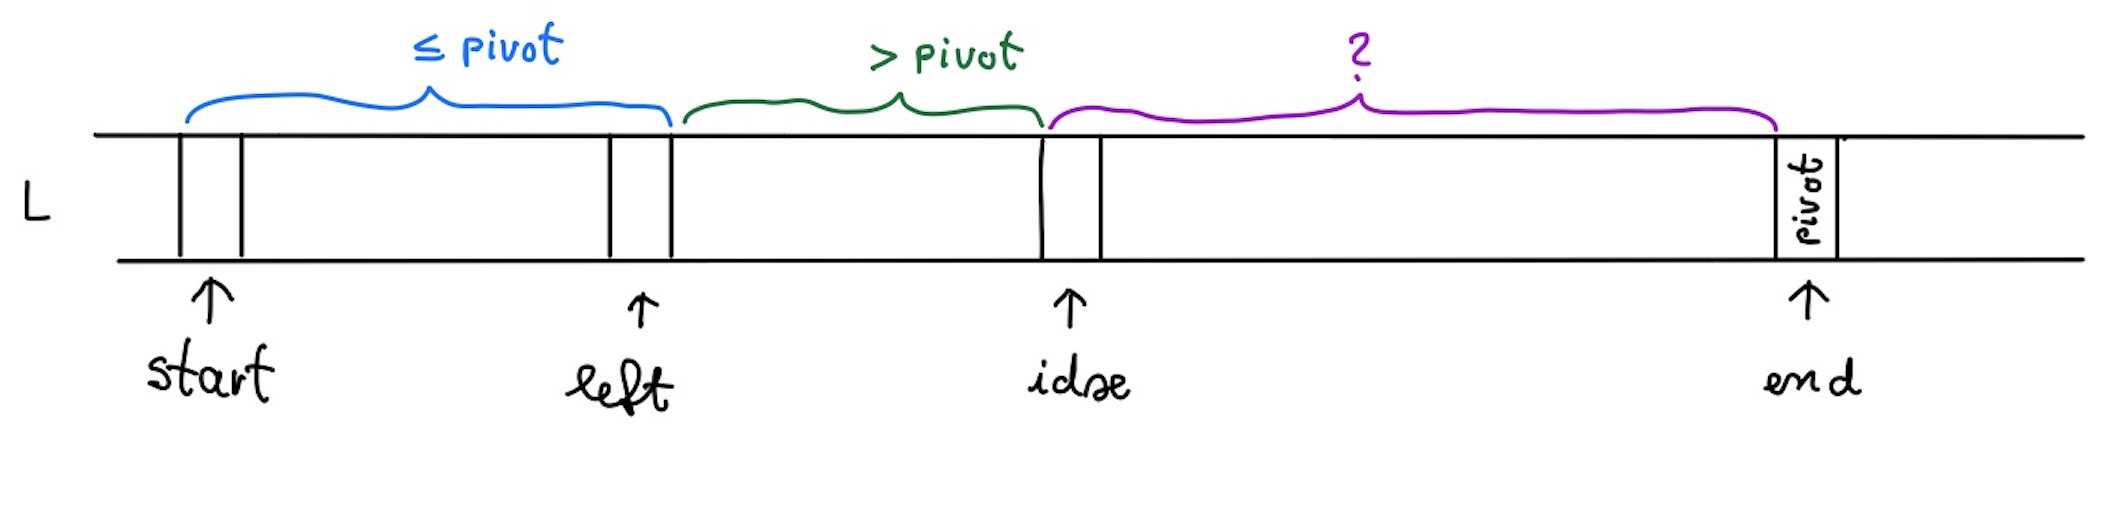
\epsfig{file=Abbildungen/lomuto.png, scale=0.40}} 
  \caption{The invariants of the function \mytt{partition}.}
  \label{fig:lomuto.png}
\end{figure}


      Observe how the invariants (a) and (b) are maintained:
      \begin{enumerate}
      \item Initially, the invariants are true because the corresponding sets are empty.
            At the start of the \mytt{for}-loop we have
            \\[0.2cm]
            \hspace*{1.3cm}
            $\{ \mytt{start}, \cdots, \mytt{left} \} = \{ \mytt{start}, \cdots, \mytt{start} - 1\} = \{\}$
            \\
            and
            \\
            \hspace*{1.3cm}
            $\{ \mytt{left}+1,\cdots,\mytt{idx}-1\} =  \{ \mytt{start},\cdots,\mytt{start}-1\}=\{\}$.
      \item If the element $\mytt{L[idx]}$ is less than the
            pivot element, it need to become part of the subarray $\mytt{L}[\mytt{start}:\mytt{left}+1]$.  In order to
            achieve this, it is placed at the position $\mytt{L}[\mytt{left}+1]$.  The element that has been at
            that position is part of the subarray $\mytt{L}[\mytt{left}+1:\mytt{idx}]$ and therefore,
            most of the times,\footnote{
              It is not always greater than the pivot element
              because the subarray $\mytt{L}[\mytt{left}+1:\mytt{idx}]$ might well be empty.}
            it is greater than the pivot element.  
            Hence we append this element to the end of the subarray
            $\mytt{L}[\mytt{left}+1:\mytt{idx}]$.  After incrementing the index $\mytt{left}$,
            both the placing of the element $\mytt{L[idx]}$ at position $\mytt{left}+1$ and the appending
            of the element $\mytt{L}[\mytt{left}+1]$ to the end of the subarray
            $\mytt{L}[\mytt{left}+1:\mytt{idx}+1]$ is achieved by the statement
            \\[0.2cm]
            \hspace*{1.3cm}
            \mytt{swap(left, idx, L)}.            
      \end{enumerate}
      Once the \mytt{for} loop in line 14 terminates, the call to $\mytt{swap}$ in line 18 moves
      the pivot element into its correct position and returns the index where the pivot element has been
      placed. 
\end{enumerate}


\subsection{Improvements for Quicksort}
There are a number of tricks that can be used to increase the efficiency of \blue{quicksort}.
\begin{enumerate}
\item Instead of taking the first element as the pivot element, use three elements from the list
      $\mytt{L}$ that is to be sorted.  For example, take the first element, the last element, and an
      element from the middle of the list.  Now compare these three elements and take that element as
      a pivot that is the \blue{median} of these elements,  where the \blue{median} \index{median} of three
      elements is defined as the element that lies between the minimum and the maximum of these elements.
      In general, the \blue{median} of a list $L$ of length $2 \cdot n +1$ is defined as the element $x$ such that at
      least $n$ elements of $L$ are less or equal to $x$ and at least $n$ elements are bigger or equal than $x$.
      
      The advantage of this strategy is that the worst case performance is much less likely to occur.  In
      particular,  using this strategy the worst case won't occur for a list that is already
      sorted.
\item If a sublist contains fewer than 10 elements, use \blue{insertion sort} to sort this sublist.

      The paper ``\blue{Engineering a Sort Function}'' by Jon L.~Bentley and M.~Douglas McIlroy
      \cite{bentley:93} describes the previous two improvements.
\item In order to be sure that the average case analysis of \blue{quicksort} holds we can randomly
      \blue{shuffle} the list $L$ that is to be sorted.  This approach is advocated by Sedgewick
      \cite{sedgewick:2011}.  In \textsl{Python} this is quite easy as
      the module \mytt{random} provides a predefined function \mytt{shuffle} that takes a list and shuffles
      it randomly in place.  For example, the code
      \\[0.2cm]
      \hspace*{1.3cm}
      \mytt{L = list(range(10)); random.shuffle(L); print(L)}
      \\[0.2cm]
      might print the result
      \\[0.2cm]
      \hspace*{1.3cm}
      \mytt{[1, 9, 8, 5, 2, 0, 6, 3, 4, 7]}.
\item In 2009, Vladimir Yaroslavskiy introduced \blue{dual pivot quicksort}
      \cite{yaroslavskiy:2009}.\index{dual pivot quicksort}
      His paper can be
      downloaded at the following address:
      \\[0.2cm]
      \hspace*{1.3cm}
      \href{http://codeblab.com/wp-content/uploads/2009/09/DualPivotQuicksort.pdf}{\mytt{http://codeblab.com/wp-content/uploads/2009/09/DualPivotQuicksort.pdf}}
      \\[0.2cm]
      The main idea of Yaroslavskiy is to use two pivot elements $p_1$ and $p_2$.  For example, we can
      define
      \\[0.2cm]
      \hspace*{1.3cm}
      $x := \mytt{L}[0]$, $y := \mytt{L}[-1]$, \quad and then define \quad $p_1 :=\min(x, y)$, $p_2 := \max(x, y)$.
      \\[0.2cm]
      Next, the list $\mytt{L}$ is split into three parts:
      \begin{enumerate}
      \item The first part contains those elements that are less than $p_1$.
      \item The second part contains those elements that are bigger or equal than $p_1$ but less or
            equal than $p_2$.
      \item The third part contains those elements that are bigger than $p_2$.
      \end{enumerate}
      Figure \ref{fig:dual-pivot-quick-sort.stlx} on page \pageref{fig:dual-pivot-quick-sort.stlx}
      shows a simple list-based implementation of \blue{dual pivot quicksort}.

      Various studies have shown that, on average, \blue{dual pivot quicksort} is faster than any other sorting
      algorithm.  For this reason, the version 1.7 of \textsl{Java} uses \blue{dual pivot quicksort}:
      \\[0.2cm]
      \hspace*{0.3cm}
      \href{http://www.docjar.com/html/api/java/util/DualPivotQuicksort.java.html}{http://www.docjar.com/html/api/java/util/DualPivotQuicksort.java.html} 
\end{enumerate}

\begin{figure}[!ht]
\centering
\begin{minted}[ frame         = lines, 
                  framesep      = 0.3cm, 
                  firstnumber   = 1,
                  bgcolor = sepia,
                  numbers       = left,
                  numbersep     = -0.3cm,
                  xleftmargin   = 0.0cm,
                  xrightmargin  = 0.0cm,
                ]{python3}
    def sort(L):
        if len(L) <= 1:
            return L
        x, y, *R   = L
        p1, p2     = min(x, y), max(x,y)
        L1, L2, L3 = partition(p1, p2, R)
        return sort(L1) + [p1] + sort(L2) + [p2] + sort(L3)
    
    def partition(p1, p2, L):
        if L == []:
            return [], [], []
        x, *R      = L
        R1, R2, R3 = partition(p1, p2, R)
        if x < p1:
            return [x] + R1, R2, R3
        if x <= p2:
            return R1, [x] + R2, R3
        else:
            return R1, R2, [x] + R3
\end{minted}
\vspace*{-0.3cm}
\caption{A list based implementation of \blue{dual pivot quicksort}.}
\label{fig:dual-pivot-quick-sort.stlx}
\end{figure}

\exercise
Implement a version of \blue{dual pivot quicksort} that is array-based instead of list-based.
\eoxs


\section{A Lower Bound for the Sorting Problem}
In this section we will show that any sorting algorithm that sorts elements by comparing them must
use at least 
\\[0.2cm]
\hspace*{1.3cm}
 $\Omega\bigl(n \cdot \log_2(n)\bigr)$ 
\\[0.2cm]
comparisons.  The important caveat here is that the sorting algorithm is not permitted to make any assumptions
on the elements of the list $L$ that is to be sorted.  The only operation that is allowed on these
elements is the use of the comparison operator ``\mytt{<}''.  Furthermore, to simplify matters let
us assume that all elements of the list $L$ are distinct.

Let us consider lists of two elements first, i.e.~assume we have
\\[0.2cm]
\hspace*{1.3cm}
$L = [a_1, a_2]$.  
\\[0.2cm]
In order to sort this list, one comparison is sufficient:
\begin{enumerate}
 \item If $a_1 < a_2$, then the list $[a_1, a_2]$ is sorted ascendingly.
 \item If $a_2 < a_1$, then the list $[a_2, a_1]$ is sorted ascendingly.
\end{enumerate}
If the list $L$ that is to be sorted has the form
\\[0.2cm]
\hspace*{1.3cm}
$L = [a_1,a_2,a_3]$,
\\[0.2cm]
then there are 6 possibilities to arrange these elements:
\\[0.2cm]
\hspace*{0.3cm}
$[a_1,a_2,a_3]$, \quad
$[a_1,a_3,a_2]$, \quad
$[a_2,a_1,a_3]$, \quad
$[a_2,a_3,a_1]$, \quad
$[a_3,a_1,a_2]$, \quad
$[a_3,a_2,a_1]$. 
\\[0.2cm]
Therefore, we need at least three comparisons, since with two comparisons we could choose between at most 
four different possibilities.  Next, we generalize this observation.

\begin{Theorem}
Given a list $L$ of $n$ different elements, there are 
\\[0.2cm]
\hspace*{1.3cm}
$\ds n! = 1 \cdot 2 \cdot 3 \cdot {\dots} \cdot (n-1) \cdot n = \prod\limits_{i=1}^n i$ 
\\[0.2cm]
different permutations of $L$. 
\end{Theorem}
\proof The claim is proven by induction on $n$. 
\begin{enumerate}
\item[B.C.:] $n=1$:  

      There is only $1$ way to arrange one element in a list.  As $1! = 1$ the claim is true in this case.
\item[I.S.:] $n \mapsto n+1$:
  
      If we have $n+1$ different elements and want to arrange these elements in a list, then there
      are $n+1$ possibilities for the first element.  In each of these cases the induction
      hypothesis tells us that there are $n!$ ways to arrange the remaining $n$ elements in a list.
      Therefore, all in all there are $(n+1) \cdot n! = (n+1)!$ different arrangements of $n+1$
      elements in a list. \qed
\end{enumerate}
Next, we consider how many different cases can be distinguished if we have $k$ different tests
that only give $\mytt{True}$ or $\mytt{False}$ answers.  Tests of this kind are called \blue{binary tests}.
\begin{enumerate}
\item If we restrict ourselves to binary tests, then one test can only distinguish between two cases.
\item If we have $2$ tests, then we can distinguish between  $2 \cdot 2 = 2^2$ different cases.
\item In general, an easy induction shows that $k$ tests can choose from at most $2^k$ different cases.
\end{enumerate}
The last claim can also be argued as follows:  If the results of the tests are represented as
$0$ and $1$, then $k$ binary tests correspond to a binary string of length
$k$.  However, binary strings of length $k$ can be used to code the numbers from $0$ up to
$2^{k}-1$.  We have
\\[0.2cm]
\hspace*{1.3cm}
$\textsl{card}\bigl(\{0,1,2,\cdots, 2^k-1\}\bigr) = 2^k$.
\\[0.2cm]
Hence there are $2^k$ binary strings of length $k$.  

If we have a list of $n$ different elements, then there are $n!$ different permutations of these
elements.  In order to figure out which of these $n!$ different permutations is given we have to
perform $k$ comparisons, where we must have
\\[0.2cm]
\hspace*{1.3cm}
$2^k \geq n!$.
\\[0.2cm]
This immediately implies
\\[0.2cm]
\hspace*{1.3cm}
$k \geq \log_2(n!)$.
\\[0.2cm]
In order to proceed, we need a lower bound for the expression $\log_2(n!)$.
First, we have
\\[0.2cm]
\hspace*{1.3cm}
$\ds \log_2(n!) = \log_2\left(\prod\limits_{i=1}^n i\right) = \sum\limits_{i=1}^n \log_2(i)$
\\[0.2cm]
The crucial idea is to interpret this sum as an upper \href{https://en.wikipedia.org/wiki/Riemann_sum}{Riemann sum}
of the integral
\\[0.2cm]
\hspace*{1.3cm}
$\ds\int_1^n\log_2(x)\, \mathrm{d}x$
\\[0.2cm]
as is shown in Figure \ref{fig:riemann-sum.pdf}\footnote{
  I have created this figure using the highly recommended tool \href{https://www.geogebra.org/m/h4P4cjsT}{geogebra}.
}.

\begin{figure}[!ht]
  \centering
  \framebox{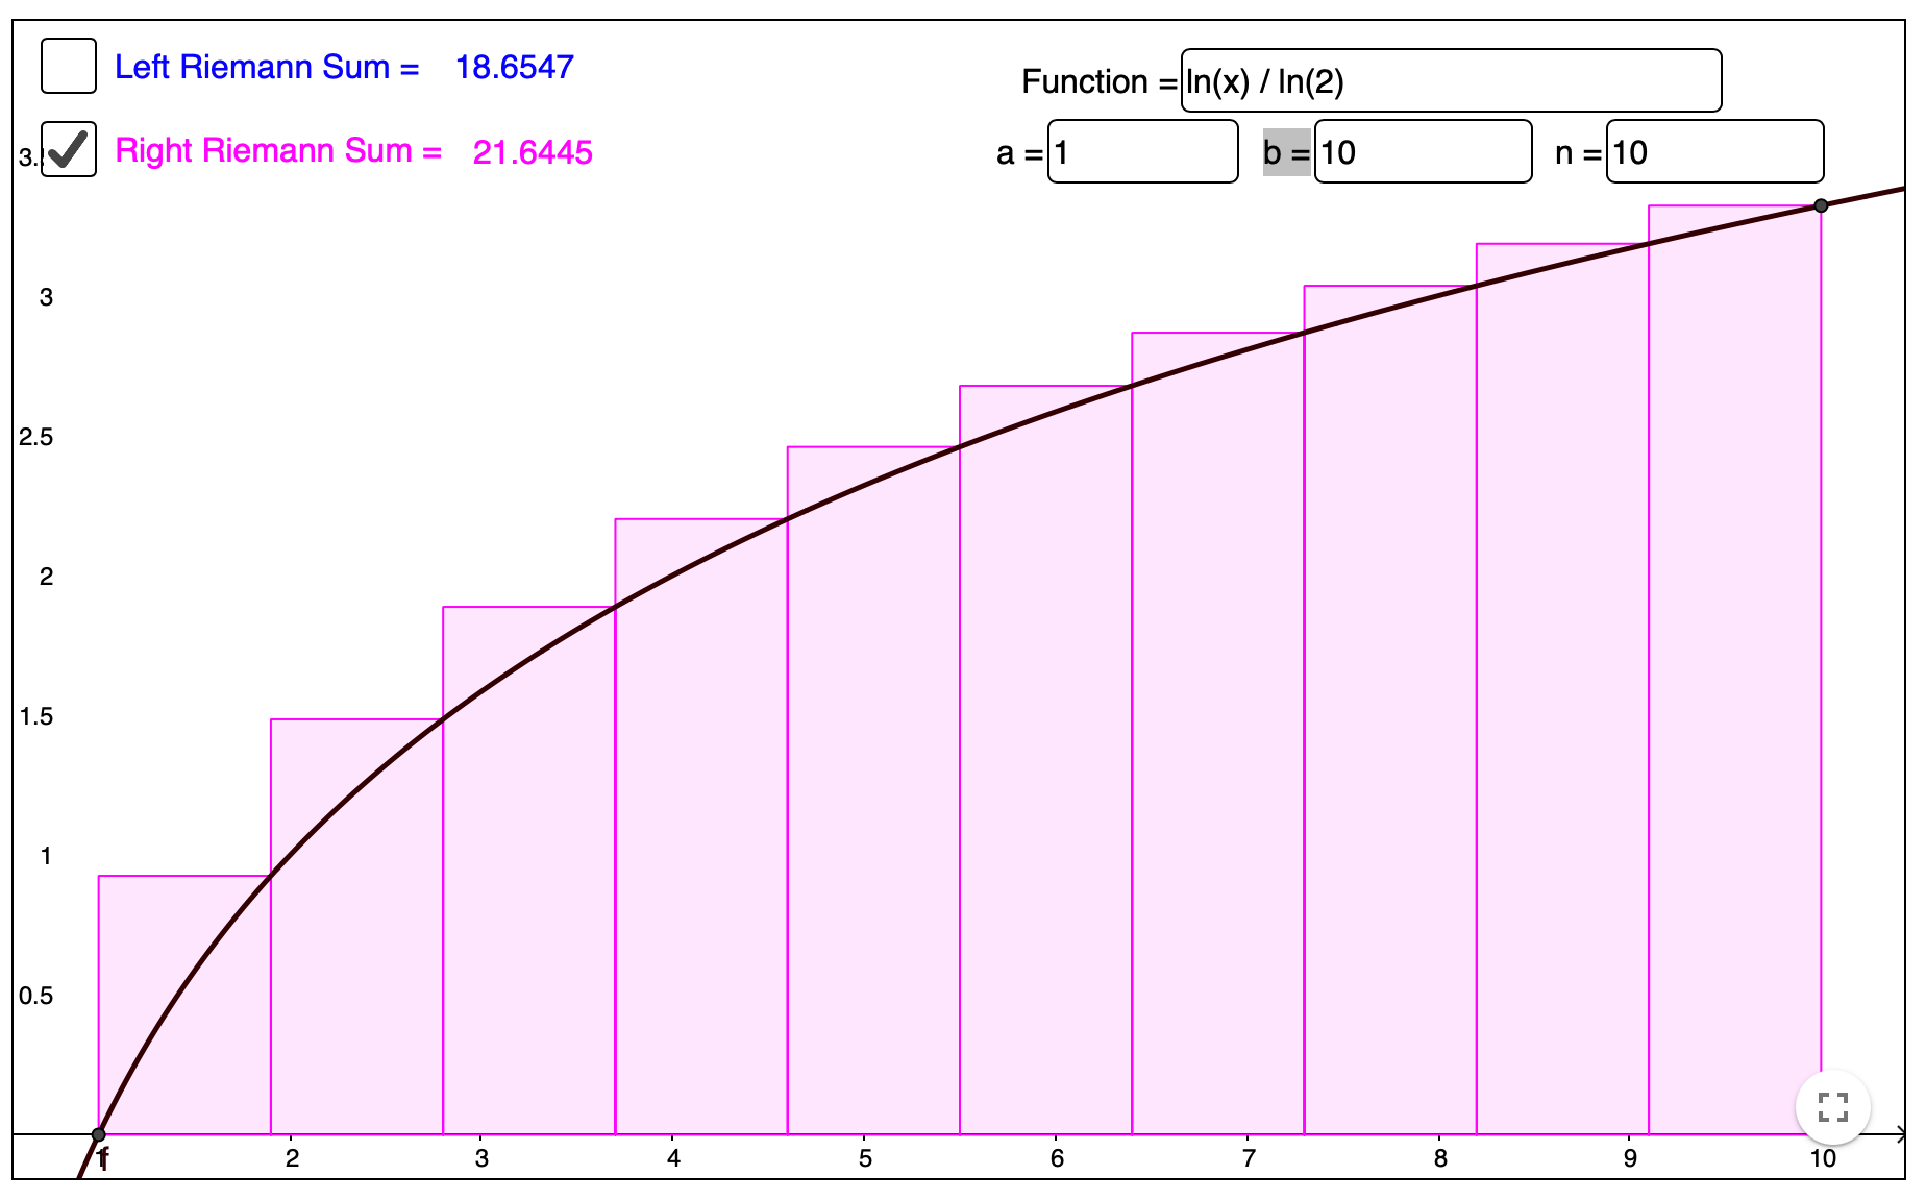
\epsfig{file=Abbildungen/riemann-sum.pdf, scale=0.45}} 
  \caption{The upper sum for the integral $\ds\int\limits_{1}^{10}\log_2(x) \,\mathrm{d}x$.}
  \label{fig:riemann-sum.pdf}
\end{figure}

Therefore we have the following chain of inequations:
\\[0.2cm]
\hspace*{1.3cm}
$
\begin{array}[t]{lcl}
  k & \geq & \ds\log_2(n!) \\[0.2cm]
    & =    & \ds\sum\limits_{i=1}^n \log_2(i) \\[0.5cm]
    & \geq & \ds\int\limits_{1}^n \log_2(x)\, \mathrm{d}x \\[0.2cm]
    & =    & \ds\frac{1}{\,\ln(2)\,} \cdot \int\limits_{1}^n \ln(x)\, \mathrm{d}x  \\[0.2cm]
    & =    & \ds\frac{1}{\,\ln(2)\,} \cdot \bigl[x \cdot \ln(x) - x \bigr]_{1}^n   \\[0.4cm]
    & =    & \ds\frac{1}{\,\ln(2)\,} \cdot \bigl(n \cdot \ln(n) - n + 1\bigr)     \\[0.2cm]
    & =    & \ds n \cdot \log_2(n) - \frac{\,n-1\,}{\,\ln(2)\,}                       
\end{array}
$ 
\\[0.2cm]
This show that
\\[0.2cm]
\hspace*{1.3cm}
$k \geq n \cdot \ds\log_2(n) - \frac{\,n-1\,}{\,\ln(2)\,}$.
\\[0.2cm]
As \blue{merge sort} is able to sort a list of length $n$ using only $n \cdot \log_2(n)$ comparisons
we have shown that this algorithm is optimal with respect to the number of comparisons within a linear bound of
size $(n-1)/\ln(2)$.




\section{Counting Sort}
\index{counting sort}
In the last section of this chapter we introduce a sorting algorithm that has only a \blue{linear} complexity.
According to the result of the previous section this algorithm can not work by comparing the elements of the
list that is to be sorted.  This algorithm only works if the elements of the list that is to be sorted are
natural numbers of a fixed size.  The algorithm is called
\href{https://en.wikipedia.org/wiki/Counting_sort}{counting sort}. We 
explain this algorithm via an example.  Table \ref{tab:marks} on page \pageref{tab:marks} shows a table showing
students and their grades.  As it stands, the names of the students are ordered alphabetically.  However, the
teacher would like to sort the list of students according to their grades.  Within a group of students that
have achieved the same grade, the students should still be ordered alphabetically.  Table
\ref{tab:marks-sorted} on page \pageref{tab:marks-sorted} shows the table that has been sorted accordingly.

\begin{table}[!ht]
  \centering
  \begin{tabular}{|l|c|}
    \hline
    Student   & Grade \\
    \hline
    \hline
    Alexander & 4 \\
    \hline
    Benjamin  & 2 \\
    \hline
    Daniel    & 3 \\
    \hline
    David     & 3 \\
    \hline
    Elijah    & 2 \\
    \hline
    Gabriel   & 1 \\
    \hline
    Henry     & 2 \\
    \hline
    Jacob     & 5 \\
    \hline
    James     & 3 \\
    \hline
    Joseph    & 2 \\
    \hline
    Liam      & 2 \\
    \hline
    Logan     & 3 \\
    \hline
    Lucas     & 1 \\
    \hline
    Mason     & 2 \\
    \hline
    Matthew   & 5 \\
    \hline
    Michael   & 3 \\
    \hline
    Noah      & 4 \\
    \hline
    Oliver    & 2 \\
    \hline
    Owen      & 4 \\
    \hline
    Samuel    & 3 \\
    \hline
    Sebastian & 2 \\
    \hline
    William   & 1 \\
    \hline
  \end{tabular}
  \caption{Students and their grades, sorted alphabetically.}
  \label{tab:marks}
\end{table}

\begin{table}[!ht]
  \centering
  \begin{tabular}{|l|c|}
    \hline
    Student   & Grade \\
    \hline
    \hline
    Gabriel   & 1 \\
    \hline
    Lucas     & 1 \\
    \hline
    William   & 1 \\
    \hline
    Benjamin  & 2 \\
    \hline
    Elijah    & 2 \\
    \hline
    Henry     & 2 \\
    \hline
    Joseph    & 2 \\
    \hline
    Liam      & 2 \\
    \hline
    Mason     & 2 \\
    \hline
    Oliver    & 2 \\
    \hline
    Sebastian & 2 \\
    \hline
    Daniel    & 3 \\
    \hline
    David     & 3 \\
    \hline
    James     & 3 \\
    \hline
    Logan     & 3 \\
    \hline
    Michael   & 3 \\
    \hline
    Samuel    & 3 \\
    \hline
    Alexander & 4 \\
    \hline
    Noah      & 4 \\
    \hline
    Owen      & 4 \\
    \hline
    Jacob     & 5 \\
    \hline
    Matthew   & 5 \\
    \hline
  \end{tabular}
  \caption{Students and their grades, sorted with respect to the grade.}
  \label{tab:marks-sorted}
\end{table}
We proceed to describe an algorithm that is capable of transforming Table \ref{tab:marks} into Table
\ref{tab:marks-sorted}.  This algorithm works in three stages.
\begin{enumerate}
\item The first stage is the \blue{counting stage}.  In this stage we count the number of students
      that have a specific grades.  In the example from Table \ref{tab:marks} we find the following:
      \begin{enumerate}[(a)]
      \item 3 students have grade 1.
      \item 8 students have grade 2.
      \item 6 students have grade 3.
      \item 3 students have grade 4.
      \item 2 students have grade 5.
      \end{enumerate}
\item The second stage is the \blue{indexing stage}.  In this stage our goal is compute the indices of the
      sublists containing the different grades.  For example, since there are 3 students with a grade of $1$
      and $1$ is the smallest grade, we know that the students with grade $1$ will be found in the sublist
      $\mytt{L[0:3]}$.  Similarly, as there are $8$ students that have a grade of $2$ and $3 + 8 = 11$,
      the sublist $\mytt{L[3:11]}$ will contain the students with grade $2$.
      All in all, we have the following:
      \begin{enumerate}[(a)]
      \item The sublist $\mytt{L[0:3]}$ contains the students with grade 1.
      \item The sublist $\mytt{L[3:11]}$ contains the students with grade 2.
      \item The sublist $\mytt{L[11:17]}$ contains the students with grade 3.
      \item The sublist $\mytt{L[17:20]}$ contains the students with grade 4.
      \item The sublist $\mytt{L[20:22]}$ contains the losers.
      \end{enumerate}
      The indexing stage computes the \blue{starting indices} of these sublists.
      Of course,  the first sublist has to start at the index $0$.  Since there are 3 students with a grade of 1,
      the second sublist starts at the index $0 + 3 = 3$.  Since there are 8 students with a grade of 2, the third
      sublist starts at the index $0 + 3 + 8 = 11$.  In general, if the sublist for the students with grade $g$
      starts at index $i_g$ and there are $n_g$ students that have achieved the grade $g$, then the sublist for the
      students with grade $g+1$ starts at index $i_{g+1}$ where
      \\[0.2cm]
      \hspace*{1.3cm}
      $\ds i_{g+1} = i_g + n_g$.
\item The \blue{distribution stage} iterates over the list of students and inserts them into the sublists
      corresponding to the grades of the students.
\end{enumerate}
Figure \ref{fig:counting-sort.stlx} on page \pageref{fig:counting-sort.stlx} shows an implementation of
counting sort.  We proceed to discuss this algorithm line by line.

\begin{figure}[!ht]
\centering
\begin{minted}[ frame         = lines, 
                  framesep      = 0.3cm, 
                  firstnumber   = 1,
                  bgcolor = sepia,
                  numbers       = left,
                  numbersep     = -0.2cm,
                  xleftmargin   = 0.8cm,
                  xrightmargin  = 0.8cm,
                ]{python3}
    def countingSort(Students):
        maxGrade =    255
        Counts   =    [0] * (maxGrade+1)
        Index    = [None] * (maxGrade+1)
        Sorted   = [None] * len(Students)
        # Phase 1: Counting
        for _name, grade in Students:
            Counts[grade] += 1
        # Phase 2: Indexing
        Index[0] = 0
        for grade in range(maxGrade):
            Index[grade+1] = Index[grade] + Counts[grade]
        # Phase 3: Distribution
        for name, grade in Students:
            idx           = Index[grade]
            Sorted[idx]   = (name, grade)
            Index[grade] += 1
        return Sorted
\end{minted}
\vspace*{-0.3cm}
\caption{An implementation of \blue{counting sort}.}
\label{fig:counting-sort.stlx}
\end{figure}

\begin{enumerate}
\item The function \mytt{countingSort} receives one argument.  The list $\mytt{Students}$
      is a list of pairs of the form $\mytt{(name, grade)}$ where
      \begin{enumerate}
      \item \mytt{name}  is the name of a student, while
      \item \mytt{grade} is the grade that this student has achieved.
      \end{enumerate}
      The list $\mytt{Students}$ is sorted alphabetically w.r.t.~the names of the students.
      The purpose of the function \mytt{countingSort} is to sort this list according to their grades.
      Sublists of students with the same grade should still be sorted alphabetically.
\item In order for our function to generalize to arbitrary numbers we will assume that all grades are elements
      of the set $\{0,\cdots,255\}$.  Therefore we define $\mytt{maxGrade}$ as $255$.
      Of course, in the example discussed so far we know that the largest
      grade is $5$.  However, we will use the function $\mytt{countingSort}$ later as an auxiliary function
      when implementing \blue{radix sort}.  Then the grades will be bytes and hence be natural numbers less
      or equal than $255$.
\item Next, we initialize the auxiliary array \mytt{Count} to be an array of length $\mytt{maxGrade}+1$.
      Later, for a grade $g$ the number $\mytt{Counts}[g]$ will contain the number of students that have
      attained the grade $g$.  Initially, all entries of the array \mytt{Count} are set to $0$.
\item After the indexing stage, the array \mytt{Index} will contain the start indices of the different sublists.
      For a grade $g$, $\mytt{Index}[g]$ is the first index of the sublist containing those students that
      have achieved the grade $g$.
\item The list \mytt{Sorted} is the list that will be returned as the result.
      This list will contain pairs of the form \mytt{(name, grade)} where \mytt{name} is the name of a student
      and \mytt{grade} is her grade.
\item The \mytt{for}-loop in line 7-8 performs the \blue{counting stage}.  We iterate over all grades
      in the list \mytt{Students} and increment the counter $\mytt{Counts}[\mytt{grade}]$ that is associated with the given grade.
\item Next, the index for the start of the sublist containing those students that have achieved the grade $0$
      is initialized as $0$ in line 10. 
\item Then, the \mytt{for}-loop in line 11-12 performs the \blue{indexing stage}. As the number
      $\mytt{Index}[\mytt{grade}]$ is the index of the start of the sublist for those students that have
      achieved the grade  $\mytt{grade}$ and the number of these
      students is $\mytt{Counts}[\mytt{grade}]$, the sublist of the students with grade $\mytt{grade}+1$
      has to start at index 
      \\[0.2cm]
      \hspace*{1.3cm}
      $\mytt{Index}[\mytt{grade}] + \mytt{Counts}[\mytt{grade}]$.
\item Finally, the \mytt{for}-loop in line 14-17 performs the \blue{distribution stage}.
      \begin{enumerate}
      \item The \mytt{for}-loop iterates over all students. 
      \item We need to find where to put a student with grade \mytt{grade}.
            $\mytt{Index}[\mytt{grade}]$ gives us the \mytt{index} of the next free entry in the
            result list \mytt{Sorted} corresponding for this grade.
      \item In line 16 the students name and her grade are stored in the result lists \mytt{Sorted}
            at the index $\mytt{idx}$.
      \item Finally, we need to increment the index stored at $\mytt{Index}[\mytt{grade}]$ since we have
            just used this index and therefore the next student with the same grade needs to be
            stored at the subsequent location.  This is done in line 17.
      \end{enumerate}
\end{enumerate}
If the list \mytt{Students} has a length of $n$, then it is easy to
see that counting sort has the complexity $\Oh(n)$.  The first \mytt{for}-loop iterates over the list \mytt{Students} so
its body is executed $n$ times.  The second for loop iterates 255 times and the last \mytt{for}-loop again
iterates $n$ times.  Hence, counting sort is a \blue{linear sorting algorithm}.  Note that we do not compare grades in
order to sort them.

Another important fact is that counting sort is \blue{stable}\index{stable}: In the resulting list, the sublists
corresponding to the different grades are still sorted alphabetically.  This is so because these sublists are
filled by iterating over the original list that is sorted alphabetically.  If two students $x$ and $y$ have the
same grade $g$ but the name of $x$ is alphabetically before the name of $y$, then $x$ will be inserted into the
sublist corresponding to grade $g$ before $y$ and hence these sublists are still ordered alphabetically.  This property
is crucial for the development of our next sorting algorithm \blue{radix sort}.

\section{Radix Sort}
\index{radix sort}
The importance of the previous sorting algorithm, \blue{counting sort}, stems from the fact that it is part of the
implementation of \href{https://en.wikipedia.org/wiki/Radix_sort}{radix sort}. \index{radix sort}
\blue{Radix sort} was used as early as 1887 in 
\href{https://en.wikipedia.org/wiki/Tabulating_machine}{tabulating machines} constructed by
\href{https://en.wikipedia.org/wiki/Herman_Hollerith}{Hermann Hollerith}.  \index{Hollerith, Herman} He was the founder of
the \blue{Tabulating Machine Company} that later became \href{https://en.wikipedia.org/wiki/IBM}{\textsc{Ibm}}.
To understand radix sort, suppose we want to implement an algorithm that sorts a large number of 32 bit
unsigned integers.  The easiest way to do this would be to use counting sort:
The main idea of radix sort is to split the
32 bit numbers into four chunks of 8 bits each and to use each of these four chunks as a grade.  To formulate this
mathematically, a 32 bit unsigned integer $x$ is defined via its four bytes $b_1$, $\cdots$, $b_4$ as follows:
\\[0.2cm]
\hspace*{1.3cm}
$\ds x = b_4 \cdot 256^{3} + b_3 \cdot 256^{2} + b_2 \cdot 256^{1} + b_1$.
\\[0.2cm]
Note that we have numbered the bytes starting from the the least significant byte.
Then, radix sort works as follows:
\begin{enumerate}
\item Sort the numbers by interpreting the byte $b_1$ as a grade.
\item Take the numbers that have been sorted by the byte $b_1$ and sort them according to the byte $b_2$ next.
      Since counting sort is \blue{stable}, numbers which happen to have the same byte $b_2$ will still be
      sorted with respect to the byte $b_1$.  Hence, after the sorting with respect to the byte $b_2$ is
      complete, in effect the numbers will then be sorted according to both $b_2$ and $b_1$.
\item Next, use counting sort to sort the numbers with respect to the byte $b_3$.
\item Finally, use counting sort to sort the numbers with respect to the byte $b_4$.  By the stability of
      counting sort, the numbers are now sorted with respect to all of their byte, where $b_4$ is the most
      significant byte and $b_1$ is the least significant byte. Hence, the numbers are sorted. 
\end{enumerate}


\begin{figure}[!ht]
\centering
\begin{minted}[ frame         = lines, 
                  framesep      = 0.3cm, 
                  firstnumber   = 1,
                  bgcolor = sepia,
                  numbers       = left,
                  numbersep     = -0.2cm,
                  xleftmargin   = 0.8cm,
                  xrightmargin  = 0.8cm,
                  ]{python3}
    def extractByte(n, k):
        return n >> (8 * (k-1)) & 0b11111111
    
    def radixSort(L):
        L = [(n, 0) for n in L]
        for k in range(1, 4+1):
            L = [(n, extractByte(n, k)) for (n, _) in L]
            L = countingSort(L)
        return [n for (n, _) in L]    
\end{minted}
\vspace*{-0.3cm}
\caption{An implementation of \blue{radix sort} for sorting unsigned 32 integers.}
\label{fig:radix-sort.stlx}
\end{figure}
Figure \ref{fig:radix-sort.stlx} on page \pageref{fig:radix-sort.stlx} shows an implementation of radix
sort that implements this idea.
\begin{enumerate}
\item The function \mytt{extractByte} is called with two arguments:
      \begin{enumerate}[(a)]
      \item $n$ is supposed to be an unsigned 32 bit number.  Hence $n$ is a integer satisfying $0 \leq n < 2^{32}$.
      \item $k$ is the index of the byte that is to be extracted.  It is supposed that the least significant
            byte has the index $1$.
      \end{enumerate}
      Hence, $\mytt{extractByte}(n, k)$ extracts the $k$-th byte of the number $n$.

      \mytt{extractByte} works by shifting the number $x$ by $(k-1) \cdot 8$ bits to the right using the shift
      operator ``\mytt{>>}''.  This shift removes all bytes with index less than $k$. Then, the least significant
      byte of the remaining number is extracted using the  \blue{bitwise and operator} ``\mytt{\&}'' with the
      mask $255$.  Note that $255$ is written as $11111111_2$ in binary and hence can be used to extract the
      eight least significant bits of a number. 
\item \mytt{radixSort} takes a list of unsigned 32 bit integers $L$ as its arguments.
\item This list is extended to a list of pairs where the first component of each pair is the number.      
\item Then \mytt{radixSort} iterates over the four bytes of the numbers of the list $L$ starting with the
      least significant byte.
\item In line 7 the $k^\mathrm{th}$ byte of the numbers of $L$ is written into the second component
      of the pairs stored in the list.      
\item With respect to \mytt{countingSort},  the elements of the list given to \mytt{countingSort} as its
      first argument are 
      arbitrary objects.  Therefore, it does not matter whether the first argument to the function
      \mytt{countingSort} is a list of strings interpreted as student names or a list of numbers.
      Therefore in line 8 this list
      is sorted with respect to the $k^\mathrm{th}$ byte. 
\item When $L$ is returned, this list is sorted with respect to all of the four bytes making up its numbers and
      hence, it is sorted.
\end{enumerate}

\section{Application: Handwritten Digit Recognition}
\index{digit recognition}
In the last section of this chapter we discuss an application of sorting:
\blue{recognizing handwritten digits}.\index{handwritten digit recognition}
We will use a \blue{training set} of $50,000$ handwritten digits. Figure \ref{fig:digits.pdf} shows the first 24
images of these handwritten digits.  These images are given as grey scale images of $28 \times 28$ pixels.
Each pixel $p$ is a floating point number satisfying $0 \leq p \leq 1$. If $p = 1.0$, the pixel is completely
black, while $p = 0.0$ if the pixel is white.  Furthermore, for each of these images we also have been given a
\blue{label} $d \in \{0,1,2,\cdots,9\}$, which specifies the digit that is represented in the image.  Besides the training set 
there is also a \blue{test set} of $10,000$ of handwritten images.  Our task is to \blue{classify} the images
of this test set as digits, i.e.~for each image of the test set we want to recognize the digit that is depicted.


\begin{figure}[!ht]
  \centering
  \framebox{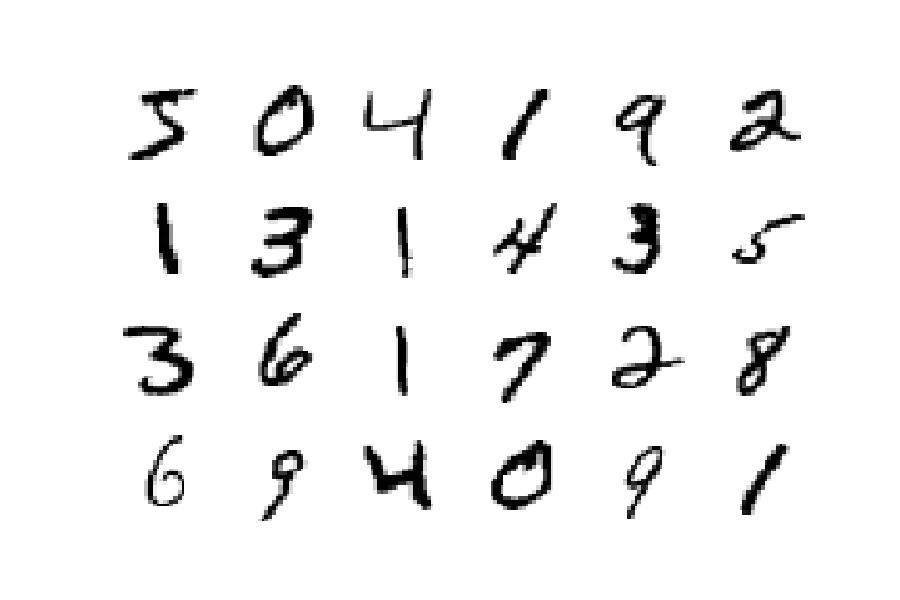
\epsfig{file=Abbildungen/digits.pdf, scale=0.60}} 
  \caption{The first 24 digits of our dataset.}
  \label{fig:digits.pdf}
\end{figure}

\subsection{The $k$-Nearest Neighbour Algorithm}
We will use the \href{https://en.wikipedia.org/wiki/K-nearest_neighbors_algorithm}{$k$-nearest neighbours algorithm} 
\index{$k$-nearest neighbours algorithm}
to solve this task.  Given an image $x$ that is to be classified as a digit, we look at those images in the
training set that are somehow \blue{close} to $x$.  If these images are all labelled with the same digit $d$,
we conclude that $x$ shows the digit $d$.  In order to implement this algorithm, we have to specify what it
means for an image $\mathbf{x}$ to be close to another image $\mathbf{y}$.  As the images have a size of $28 \times 28 = 784$
pixels, they can be viewed as $784$-dimensional vectors.  We can compute the \blue{Euclidean distance}
$d(\mathbf{x}, \mathbf{y})$ between $\mathbf{x}$ and $\mathbf{y}$ using the formula
\\[0.2cm]
\hspace*{1.3cm}
$\ds d(\mathbf{x}, \mathbf{y}) := \sqrt{\sum\limits_{i=1}^n (x_i - y_i)^2\;}$.
\\[0.2cm]
This formula is a generalization of the distance between two points $(x_1, x_2)$ and $(y_1, y_2)$ in the the
plane $\mathbb{R}^2$, which, according to the \href{https://en.wikipedia.org/wiki/Pythagorean_theorem}{Pythagorean theorem}, is given as 
\\[0.2cm]
\hspace*{1.3cm}
$\sqrt{(x_1 - y_1)^2 + (x_2 - y_2)^2\;}$.
\\[0.2cm]
Given an image $\mathbf{y}$ that needs to be classified and a training set of $n$ labelled images, the $k$-nearest
neighbours algorithm works as follows: 
\begin{enumerate}[(a)]
\item For every image $\mathbf{x}$ in the training set compute the Euclidean distance $d(\mathbf{x},
  \mathbf{y})$ between $\mathbf{x}$ and $\mathbf{y}$.
\item \blue{Sort} the images in the training set according to their distance to $\mathbf{y}$.
\item Pick those $k$ images that have the smallest distances to $\mathbf{y}$.
      These $k$ images are called the \blue{$k$ nearest neighbours}.
\item Among the $k$ nearest neighbours, pick the label that occurs most frequently.
      
      For example, if $k=7$ and $3$ of the $7$ nearest neighbours are labelled as the digit $3$, while $2$ are
      labelled as the digit $2$ and $2$ are labelled as the digit $1$, then we conclude that the image
      $\mathbf{y}$ shows the digit $3$. 
\end{enumerate}

\begin{figure}[!ht]
\centering
\begin{minted}[ frame         = lines, 
                 framesep      = 0.3cm, 
                 firstnumber   = 1,
                 bgcolor       = sepia,
                 numbers       = left,
                 numbersep     = -0.3cm,
                 xleftmargin   = 0.0cm,
                 xrightmargin  = 0.0cm,
               ]{python3}
    import gzip
    import pickle
    import numpy as np

    def load_data():
        with gzip.open('mnist.pkl.gz', 'rb') as f:
            train, _, test = pickle.load(f, encoding="latin1")
        return (train[0], test[0], train[1], test[1])
        
    X_train, X_test, Y_train, Y_test = load_data()
        
    def distance(x, y):
        return np.sqrt(np.sum((x - y)**2))
    
    def maxCount(L):
        Frequencies         = {}    # number of occurrences 
        most_frequent       = L[0]  # most frequent digit so far
        most_frequent_count = 1     
        for d in L:
            if d in Frequencies:
                Frequencies[d] += 1
            else:
                Frequencies[d]  = 1
            if Frequencies[d] > most_frequent_count:
                most_frequent       = d
                most_frequent_count = Frequencies[d]
        return most_frequent, most_frequent_count / len(L)
    
    def digit(x, k):
        n          = X_train.shape[0]  # number of all training images
        Distances  = [(distance(X_train[i,:], x), i) for i in range(n)]
        Neighbours = [Y_train[i] for _, i in sorted(Distances)]
        return maxCount(Neighbours[:k])

    digit(X_test[0,:], 13)
\end{minted}
\vspace*{-0.3cm}
\caption{The $k$-nearest neighbours algorithm for digit recognition.}
\label{fig:Digit-Recognition.ipynb}
\end{figure}

\noindent
Figure \ref{fig:Digit-Recognition.ipynb} on page \pageref{fig:Digit-Recognition.ipynb} shows a program that can
be used to recognize a handwritten digit.
\begin{enumerate}
\item The images of the handwritten digits are stored in the file \mytt{mnist.pkl.gz}.  This file is compressed
      using \mytt{gzip} and the images have been \blue{pickled} using the module
      \mytt{pickle}\index{pickle}.  The module
      \mytt{pickle} supports the reading and writing of \textsl{Python} data structures and is therefore
      used to make data \blue{persistent}, i.e.~to store the data structures of a program in a file system.
      The counterpart of the function \mytt{load} is the function \mytt{dump}.

      In order to read the images of the handwritten digits, we therefore have to import the modules
      \mytt{gzip} and \mytt{pickle}.  The module \mytt{numpy} is needed as these images are stored as
      \mytt{numpy} \blue{arrays}.  
\item The function $\mytt{load\_data}()$ returns a tuple of the form
      \\[0.2cm]
      \hspace*{1.3cm}
      $ \ds (\mytt{X\_train}, \mytt{X\_test}, \mytt{Y\_train}, \mytt{Y\_test}) $
      \\[0.2cm]
      where 
      \begin{enumerate}[(a)]
      \item $\mytt{X\_train}$ is a matrix storing the 50,000 training images of handwritten digits.
            For each $i \in \{0,\cdots,49\,999\}$ the row $\mytt{X\_train}[i, :]$ is an array of size $784$ storing a single image.
      \item $\mytt{X\_test}$ is a matrix containing 10,000 images of handwritten digits that we will use to
            test our implementation.
      \item $\mytt{Y\_train}$ is an array of size 50,000. For each $i \in \{0,\cdots,49\,999\}$ the number $\mytt{Y\_train}[i]$
            specifies the digit shown in the $i$th training image.
      \item $\mytt{Y\_test}$ is an array of size 10,000. For each $i \in \{0,\cdots,9\,999\}$ the number $\mytt{Y\_test}[i]$
            specifies the digit shown in the $i^{\mathrm{th}}$ test image.
      \end{enumerate}
      The function \mytt{open} from the module \mytt{gzip} opens the specified file and automatically
      decompresses it.  In the file \mytt{mnist.pkl.gz} the data is stored as a triple of pairs.
      For our purposes, we only need the first and the last component of this triple.  Each of these components
      is a pair of the form $(\textsl{data}, \textsl{label})$, where \textsl{data} is an array of images and
      \textsl{labels} is an array specifying the digits represented in these images.
      The function \mytt{load\_data} extracts the data stored in these pairs.
\item The function $\mytt{distance}(x, y)$ computes the Euclidean distance between the images $x$ and $y$.
      Given a vector $x$, the expression $x \mytt{**} 2$ computes a vector containing the squares of the
      components of $x$.  These squares can then be summed using the \mytt{numpy} function \mytt{sum}.
\item Given a list $L$ of digits, the function $\mytt{maxCounts}(L)$ returns a pair $(d, p)$ where $d$ is the digit that occurs most frequently in $L$
      and $p$ is the fraction of occurrences of $d$ in $L$.  For example, we have
      \\[0.2cm]
      \hspace*{1.3cm}
      $\mytt{maxCounts}([5,2,3,5,2,5,6,5,7,8]) = (5, 0.4)$
      \\[0.2cm]
      because the digit $5$ is the most frequent digit in the list $[5,2,3,5,2,5,6,5,7,8]$ and $40$\%
      of the digits in this list are fives.  In detail, the function \mytt{maxCounts} works as follows:
      \begin{enumerate}[(a)]
      \item \mytt{Frequencies} is a dictionary that specifies how often a digit $d$ occurs in the list $L$.
      \item \mytt{most\_frequent} is the digit that so far is known to be the most frequent digit in $L$.
            Initially, this is assumed to be the first digit.  As we iterate over the list $L$, this variable
            is updated.
      \item \mytt{most\_frequent\_count} is the number of occurrences of the digit \mytt{most\_frequent}.
      \item As we iterate over the digits in $L$ we update their frequencies.  If we encounter a digit that is
            more common than the digit stored in the variable \mytt{most\_frequent} we update this variable
            and the associated value \mytt{most\_frequent\_count}.
      \end{enumerate}
\item Given an image of a digit stored in the vector $\mathbf{x}$ and a number of neighbours $k$, the function
      $\mytt{digit}(\mathbf{x}, k)$ computes those $k$ images in the training set \mytt{X\_train} that are
      \blue{closest} to the image $\mathbf{x}$, where \blue{closeness} of images is defined in terms of the
      \blue{Euclidean distance} of the vectors that store these images.  From these $k$ closest images of the training
      set the function chooses the digit that occurs most frequently.  It returns a pair $(d, p)$ where $d$
      is the digit that is most frequently occurring in the list of $k$ neighbours and $p$ is the percentage
      of images in the $k$ neighbours of $\mathbf{x}$ that show the digit $d$.  The implementation works as follows:
      \begin{enumerate}[(a)]
      \item \mytt{n} is the number of training examples.  In our case, $n = 50,000$.
      \item \mytt{Distances} is a list of pairs of the form $(d, i)$, where $d$ is the distance
            of the $i$-th image in the training set from the given image $x$.
      \item These pairs are \blue{sorted} with respect to their distance and the labels corresponding to the
            images are computed.  Therefore, \mytt{Neighbours} is a list of the labels of all $50,000$
            training images sorted according to their distance to the given image $x$.
      \item Finally, the function \mytt{maxCounts} takes the $k$ closest images and computes the digit that
            is most frequently occurring.
      \end{enumerate}
\item The last line shows how the function \mytt{digit} can be used to classify the first image from the test
      set using the 13 closest neighbours. 
\end{enumerate}
\pagebreak

\exercise
In the program shown in Figure \ref{fig:Digit-Recognition.ipynb} on page \pageref{fig:Digit-Recognition.ipynb}
we have sorted the list \mytt{Distances} in line 32.  The only reason to do this was to be able to find the $k$ smallest
distances in this list.  As $k$ is a small number and the list \mytt{Distances} is rather large, this seems wasteful.
\begin{enumerate}[(a)]
\item Devise an algorithm Quickselect that selects the $k$ smallest elements from a list $L$.

      \hint
      Try to adapt the algorithm Quicksort so that instead of sorting the list it finds the $k$ smallest elements.      
\item Analyse the average complexity of your algorithm.

      \hint
      The recurrence equation resulting from an efficient implementation of Quickselect is quite complicated.
      Instead of solving this recurrence equation it is sufficient if you are able to prove by induction on the
      length $n$ of the list $L$ that your algorithm uses at most $4 \cdot n$ comparisons in order to compute
      the $k$ smallest elements.
      \eox
\end{enumerate}   
\pagebreak

\section{Check Your Understanding}
If you are able to answer the questions below confidently, then you can assume that you have mastered the concepts
introduced in this chapter.
\begin{enumerate}
\item How have we defined the concept of a \blue{linear order}?
\item What type of order do we need if we have to sort a list?
\item Describe the algorithm \blue{insertion sort} on an abstract mathematical level.
\item What is the complexity of \blue{insertion sort}?
\item Is there a case where \blue{insertion sort}  has only a linear complexity?
\item Describe the algorithm \blue{selection sort} on an abstract mathematical level.
\item What is the complexity of \blue{selection sort}?
\item Compare the complexity of \blue{selection sort} with the complexity of \blue{insertion sort}.
\item Describe the algorithm \blue{merge sort} on an abstract mathematical level.
\item Describe an array-based, non-recursive implementation of \blue{merge sort}.
\item Describe the algorithm \blue{quicksort} on an abstract mathematical level.
\item Describe an array-based implementation of \blue{quicksort}.
\item Compare the complexity of \blue{merge sort} with the complexity of \blue{quicksort}.
\item Compare the memory requierements of \blue{merge sort} and \blue{quicksort}.
\item Describe \blue{dual pivot quicksort}.
\item In which case is \blue{dual pivot quicksort} much faster than \blue{quicksort}?
\item How does \blue{counting sort} work?
\item How does \blue{radix sort} work?
\item What is the complexity of \blue{radix sort}?
\item How does the \blue{$k$-nearest neighbours algorithm} work?
\end{enumerate}

%%% Local Variables: 
%%% mode: latex
%%% TeX-master: "algorithms"
%%% End: 
